%
% file: localoperator.tex
% author: Victor Brena
% description: Briefly describes properties of the local operator.
%

\chapter{Appendix A: Universe Dataset Analysis}
\label{app:app01}

%%%%%%%%%%%%%%%%%%%%%%%%%%%%%%%%%%%%%%%%%%%%%%%%%%%%%%%%%%%%
\section{A.1 Descriptive Statistics}
%%%%%%%%%%%%%%%%%%%%%%%%%%%%%%%%%%%%%%%%%%%%%%%%%%%%%%%%%%%%


%%%%%%%%%%%%%%%%%%%%%%%%%%%%%%%%%%%%%%%%%%%%%%%%%%%%%%%%%%%%
\subsection{A.1.1 Summary Statistics}
%%%%%%%%%%%%%%%%%%%%%%%%%%%%%%%%%%%%%%%%%%%%%%%%%%%%%%%%%%%%


%%%%%%%%%%%%%%%%%%%%%%%%%%%%%%%%%%%%%%%%%%%%%%%%%%%%%%%%%%%%
%\subsubsection{A.1.1.1 Green Bonds}
%%%%%%%%%%%%%%%%%%%%%%%%%%%%%%%%%%%%%%%%%%%%%%%%%%%%%%%%%%%%

\begin{table}[!htbp] \centering 
  \caption{Universe Green Bond Summary Statistics} 
  \label{desc1} 
  \footnotesize
\begin{tabular}{@{\extracolsep{5pt}}lccccccc} 
\\[-1.8ex]\hline 
\hline \\[-1.8ex] 
Statistic & \multicolumn{1}{c}{N} & \multicolumn{1}{c}{Mean} & \multicolumn{1}{c}{St. Dev.} & \multicolumn{1}{c}{Min} & \multicolumn{1}{c}{Pctl(25)} & \multicolumn{1}{c}{Pctl(75)} & \multicolumn{1}{c}{Max} \\ 
\hline \\[-1.8ex] 
Time to Maturity (Days) & 1,024 & 3,214.172 & 2,417.984 & 367 & 1,834 & 3,660 & 21,922 \\ 
Issue Amount & 1,024 & 1,290.146 & 1,960.483 & 500 & 577.3 & 1,178.9 & 33,564 \\ 
Coupon Rate & 1,024 & 1.644 & 1.517 & 0 & 0.5 & 2.4 & 10 \\ 
Guarantor & 1,024 & 0.182 & 0.386 & 0 & 0 & 0 & 1 \\ 
Offer Yield to Maturity & 1,024 & 1.688 & 1.521 & $-$0 & 0.5 & 2.5 & 10 \\ 
2008 & 1,024 & 0.000 & 0.000 & 0 & 0 & 0 & 0 \\ 
2009 & 1,024 & 0.003 & 0.054 & 0 & 0 & 0 & 1 \\ 
2010 & 1,024 & 0.005 & 0.070 & 0 & 0 & 0 & 1 \\ 
2011 & 1,024 & 0.000 & 0.000 & 0 & 0 & 0 & 0 \\ 
2012 & 1,024 & 0.007 & 0.082 & 0 & 0 & 0 & 1 \\ 
2013 & 1,024 & 0.015 & 0.120 & 0 & 0 & 0 & 1 \\ 
2014 & 1,024 & 0.011 & 0.103 & 0 & 0 & 0 & 1 \\ 
2015 & 1,024 & 0.038 & 0.191 & 0 & 0 & 0 & 1 \\ 
2016 & 1,024 & 0.043 & 0.203 & 0 & 0 & 0 & 1 \\ 
2017 & 1,024 & 0.063 & 0.244 & 0 & 0 & 0 & 1 \\ 
2018 & 1,024 & 0.074 & 0.262 & 0 & 0 & 0 & 1 \\ 
2019 & 1,024 & 0.120 & 0.325 & 0 & 0 & 0 & 1 \\ 
2020 & 1,024 & 0.164 & 0.371 & 0 & 0 & 0 & 1 \\ 
2021 & 1,024 & 0.272 & 0.445 & 0 & 0 & 1 & 1 \\ 
2022 & 1,024 & 0.185 & 0.388 & 0 & 0 & 0 & 1 \\ 
AAA & 1,024 & 0.248 & 0.432 & 0 & 0 & 0 & 1 \\ 
AA & 1,024 & 0.181 & 0.385 & 0 & 0 & 0 & 1 \\ 
A & 1,024 & 0.242 & 0.429 & 0 & 0 & 0 & 1 \\ 
BBB & 1,024 & 0.272 & 0.445 & 0 & 0 & 1 & 1 \\ 
BB & 1,024 & 0.042 & 0.201 & 0 & 0 & 0 & 1 \\ 
B & 1,024 & 0.014 & 0.116 & 0 & 0 & 0 & 1 \\ 
CCC & 1,024 & 0.001 & 0.031 & 0 & 0 & 0 & 1 \\ 
Annual Coupon & 1,024 & 0.617 & 0.486 & 0 & 0 & 1 & 1 \\ 
Semi Annual Coupon & 1,024 & 0.380 & 0.486 & 0 & 0 & 1 & 1 \\ 
Quarterly & 1,024 & 0.002 & 0.044 & 0 & 0 & 0 & 1 \\ 
Monthly & 1,024 & 0.000 & 0.000 & 0 & 0 & 0 & 0 \\ 
Variable & 1,024 & 0.000 & 0.000 & 0 & 0 & 0 & 0 \\ 
Maturity & 1,024 & 0.001 & 0.031 & 0 & 0 & 0 & 1 \\ 
\hline \\[-1.8ex] 
\end{tabular} 
\end{table}

\begin{table}[!htbp] \centering 
  \caption{Universe Green Bond Summary Statistics cont.} 
  \label{} 
  \footnotesize
\begin{tabular}{@{\extracolsep{5pt}}lccccccc} 
\\[-1.8ex]\hline 
\hline \\[-1.8ex] 
Statistic & \multicolumn{1}{c}{N} & \multicolumn{1}{c}{Mean} & \multicolumn{1}{c}{St. Dev.} & \multicolumn{1}{c}{Min} & \multicolumn{1}{c}{Pctl(25)} & \multicolumn{1}{c}{Pctl(75)} & \multicolumn{1}{c}{Max} \\ 
\hline \\[-1.8ex] 
Academic \& Educational Services & 1,024 & 0.000 & 0.000 & 0 & 0 & 0 & 0 \\ 
Basic Materials & 1,024 & 0.021 & 0.142 & 0 & 0 & 0 & 1 \\ 
Consumer Cyclicals & 1,024 & 0.018 & 0.131 & 0 & 0 & 0 & 1 \\ 
Consumer Non-Cyclicals & 1,024 & 0.016 & 0.124 & 0 & 0 & 0 & 1 \\ 
Energy & 1,024 & 0.014 & 0.116 & 0 & 0 & 0 & 1 \\ 
Financials & 1,024 & 0.478 & 0.500 & 0 & 0 & 1 & 1 \\ 
Government Activity & 1,024 & 0.146 & 0.353 & 0 & 0 & 0 & 1 \\ 
Healthcare & 1,024 & 0.007 & 0.082 & 0 & 0 & 0 & 1 \\ 
Industrials & 1,024 & 0.057 & 0.231 & 0 & 0 & 0 & 1 \\ 
Institutions, Associations \& Organizations & 1,024 & 0.064 & 0.246 & 0 & 0 & 0 & 1 \\ 
Real Estate & 1,024 & 0.035 & 0.184 & 0 & 0 & 0 & 1 \\ 
Technology & 1,024 & 0.021 & 0.145 & 0 & 0 & 0 & 1 \\ 
Utilities & 1,024 & 0.125 & 0.331 & 0 & 0 & 0 & 1 \\ 
AUD & 1,024 & 0.004 & 0.062 & 0 & 0 & 0 & 1 \\ 
BRL & 1,024 & 0.000 & 0.000 & 0 & 0 & 0 & 0 \\ 
CAD & 1,024 & 0.019 & 0.135 & 0 & 0 & 0 & 1 \\ 
CLP & 1,024 & 0.001 & 0.031 & 0 & 0 & 0 & 1 \\ 
CNY & 1,024 & 0.001 & 0.031 & 0 & 0 & 0 & 1 \\ 
COP & 1,024 & 0.000 & 0.000 & 0 & 0 & 0 & 0 \\ 
HRK & 1,024 & 0.000 & 0.000 & 0 & 0 & 0 & 0 \\ 
EUR & 1,024 & 0.568 & 0.496 & 0 & 0 & 1 & 1 \\ 
GBP & 1,024 & 0.028 & 0.166 & 0 & 0 & 0 & 1 \\ 
HKD & 1,024 & 0.001 & 0.031 & 0 & 0 & 0 & 1 \\ 
JPY & 1,024 & 0.013 & 0.112 & 0 & 0 & 0 & 1 \\ 
KZT & 1,024 & 0.000 & 0.000 & 0 & 0 & 0 & 0 \\ 
MXN & 1,024 & 0.000 & 0.000 & 0 & 0 & 0 & 0 \\ 
NZD & 1,024 & 0.002 & 0.044 & 0 & 0 & 0 & 1 \\ 
NOK & 1,024 & 0.001 & 0.031 & 0 & 0 & 0 & 1 \\ 
PEN & 1,024 & 0.000 & 0.000 & 0 & 0 & 0 & 0 \\ 
PHP & 1,024 & 0.000 & 0.000 & 0 & 0 & 0 & 0 \\ 
RUB & 1,024 & 0.001 & 0.031 & 0 & 0 & 0 & 1 \\ 
SGD & 1,024 & 0.000 & 0.000 & 0 & 0 & 0 & 0 \\ 
SEK & 1,024 & 0.009 & 0.093 & 0 & 0 & 0 & 1 \\ 
CHF & 1,024 & 0.000 & 0.000 & 0 & 0 & 0 & 0 \\ 
THB & 1,024 & 0.000 & 0.000 & 0 & 0 & 0 & 0 \\ 
TRY & 1,024 & 0.000 & 0.000 & 0 & 0 & 0 & 0 \\ 
USD & 1,024 & 0.352 & 0.478 & 0 & 0 & 1 & 1 \\ 
UYU & 1,024 & 0.001 & 0.031 & 0 & 0 & 0 & 1 \\ 
First-Lien Loan & 1,024 & 0.003 & 0.054 & 0 & 0 & 0 & 1 \\ 
First Mortgage & 1,024 & 0.015 & 0.120 & 0 & 0 & 0 & 1 \\ 
First Refunding Mortgage & 1,024 & 0.001 & 0.031 & 0 & 0 & 0 & 1 \\ 
Second-Lien Loan & 1,024 & 0.000 & 0.000 & 0 & 0 & 0 & 0 \\ 
Junior Subordinated & 1,024 & 0.003 & 0.054 & 0 & 0 & 0 & 1 \\ 
Senior Secured Mortgage & 1,024 & 0.047 & 0.211 & 0 & 0 & 0 & 1 \\ 
Refunding Mortgage & 1,024 & 0.002 & 0.044 & 0 & 0 & 0 & 1 \\ 
Senior Secured & 1,024 & 0.045 & 0.207 & 0 & 0 & 0 & 1 \\ 
Senior Unsecured & 1,024 & 0.762 & 0.426 & 0 & 1 & 1 & 1 \\ 
Senior Non-Preferred & 1,024 & 0.041 & 0.198 & 0 & 0 & 0 & 1 \\ 
Senior Preferred & 1,024 & 0.049 & 0.216 & 0 & 0 & 0 & 1 \\ 
Senior Subordinated Unsecured & 1,024 & 0.001 & 0.031 & 0 & 0 & 0 & 1 \\ 
Senior Subordinated Secured & 1,024 & 0.000 & 0.000 & 0 & 0 & 0 & 0 \\ 
Subordinated Unsecured & 1,024 & 0.005 & 0.070 & 0 & 0 & 0 & 1 \\ 
Subordinated Secured & 1,024 & 0.000 & 0.000 & 0 & 0 & 0 & 0 \\ 
Unsecured & 1,024 & 0.024 & 0.154 & 0 & 0 & 0 & 1 \\ 
Public Sector & 1,024 & 0.361 & 0.481 & 0 & 0 & 1 & 1 \\ 
Corporate Sector & 1,024 & 0.639 & 0.481 & 0 & 0 & 1 & 1 \\ 
\hline \\[-1.8ex] 
\end{tabular} 
\end{table}

%%%%%%%%%%%%%%%%%%%%%%%%%%%%%%%%%%%%%%%%%%%%%%%%%%%%%%%%%%%%
%\subsubsection{A.1.1.2 Brown Bonds}
%%%%%%%%%%%%%%%%%%%%%%%%%%%%%%%%%%%%%%%%%%%%%%%%%%%%%%%%%%%%

\begin{table}[!htbp] \centering 
  \caption{Universe Brown Bond Summary Statistics} 
  \label{} 
  \footnotesize
\begin{tabular}{@{\extracolsep{5pt}}lccccccc} 
\\[-1.8ex]\hline 
\hline \\[-1.8ex] 
Statistic & \multicolumn{1}{c}{N} & \multicolumn{1}{c}{Mean} & \multicolumn{1}{c}{St. Dev.} & \multicolumn{1}{c}{Min} & \multicolumn{1}{c}{Pctl(25)} & \multicolumn{1}{c}{Pctl(75)} & \multicolumn{1}{c}{Max} \\ 
\hline \\[-1.8ex] 
Time to Maturity (Days) & 11,179 & 2,680.561 & 2,347.479 & 366 & 1,712 & 3,656 & 36,533 \\ 
Issue Amount & 11,179 & 1,463 & 1,409 & 500 & 673 & 1,603 & 30,089 \\ 
Coupon Rate & 11,179 & 2.688 & 1.961 & 0 & 1.1 & 3.9 & 20 \\ 
Guarantor & 11,179 & 0.240 & 0.427 & 0 & 0 & 0 & 1 \\ 
Offer Yield to Maturity & 11,179 & 2.720 & 1.969 & 0 & 1.1 & 4.0 & 20 \\ 
2008 & 11,179 & 0.059 & 0.235 & 0 & 0 & 0 & 1 \\ 
2009 & 11,179 & 0.091 & 0.287 & 0 & 0 & 0 & 1 \\ 
2010 & 11,179 & 0.084 & 0.277 & 0 & 0 & 0 & 1 \\ 
2011 & 11,179 & 0.080 & 0.271 & 0 & 0 & 0 & 1 \\ 
2012 & 11,179 & 0.093 & 0.291 & 0 & 0 & 0 & 1 \\ 
2013 & 11,179 & 0.076 & 0.266 & 0 & 0 & 0 & 1 \\ 
2014 & 11,179 & 0.076 & 0.265 & 0 & 0 & 0 & 1 \\ 
2015 & 11,179 & 0.073 & 0.259 & 0 & 0 & 0 & 1 \\ 
2016 & 11,179 & 0.068 & 0.252 & 0 & 0 & 0 & 1 \\ 
2017 & 11,179 & 0.061 & 0.240 & 0 & 0 & 0 & 1 \\ 
2018 & 11,179 & 0.056 & 0.230 & 0 & 0 & 0 & 1 \\ 
2019 & 11,179 & 0.062 & 0.242 & 0 & 0 & 0 & 1 \\ 
2020 & 11,179 & 0.047 & 0.211 & 0 & 0 & 0 & 1 \\ 
2021 & 11,179 & 0.039 & 0.193 & 0 & 0 & 0 & 1 \\ 
2022 & 11,179 & 0.035 & 0.183 & 0 & 0 & 0 & 1 \\ 
AAA & 11,179 & 0.364 & 0.481 & 0 & 0 & 1 & 1 \\ 
AA & 11,179 & 0.225 & 0.418 & 0 & 0 & 0 & 1 \\ 
A & 11,179 & 0.189 & 0.392 & 0 & 0 & 0 & 1 \\ 
BBB & 11,179 & 0.160 & 0.367 & 0 & 0 & 0 & 1 \\ 
BB & 11,179 & 0.038 & 0.191 & 0 & 0 & 0 & 1 \\ 
B & 11,179 & 0.021 & 0.142 & 0 & 0 & 0 & 1 \\ 
CCC & 11,179 & 0.003 & 0.050 & 0 & 0 & 0 & 1 \\ 
Annual Coupon & 11,179 & 0.583 & 0.493 & 0 & 0 & 1 & 1 \\ 
Semi Annual Coupon & 11,179 & 0.413 & 0.492 & 0 & 0 & 1 & 1 \\ 
Quarterly & 11,179 & 0.002 & 0.045 & 0 & 0 & 0 & 1 \\ 
Monthly & 11,179 & 0.0002 & 0.013 & 0 & 0 & 0 & 1 \\ 
Variable & 11,179 & 0.0001 & 0.009 & 0 & 0 & 0 & 1 \\ 
Maturity & 11,179 & 0.002 & 0.041 & 0 & 0 & 0 & 1 \\ 
Academic \& Educational Services & 11,179 & 0.0001 & 0.009 & 0 & 0 & 0 & 1 \\ 
Basic Materials & 11,179 & 0.012 & 0.111 & 0 & 0 & 0 & 1 \\ 
Consumer Cyclicals & 11,179 & 0.017 & 0.130 & 0 & 0 & 0 & 1 \\ 
Consumer Non-Cyclicals & 11,179 & 0.014 & 0.115 & 0 & 0 & 0 & 1 \\ 
Energy & 11,179 & 0.013 & 0.111 & 0 & 0 & 0 & 1 \\ 
Financials & 11,179 & 0.689 & 0.463 & 0 & 0 & 1 & 1 \\ 
Government Activity & 11,179 & 0.170 & 0.376 & 0 & 0 & 0 & 1 \\ 
Healthcare & 11,179 & 0.003 & 0.052 & 0 & 0 & 0 & 1 \\ 
Industrials & 11,179 & 0.024 & 0.153 & 0 & 0 & 0 & 1 \\ 
Institutions, Associations \& Organizations & 11,179 & 0.020 & 0.140 & 0 & 0 & 0 & 1 \\ 
Real Estate & 11,179 & 0.003 & 0.052 & 0 & 0 & 0 & 1 \\ 
Technology & 11,179 & 0.016 & 0.124 & 0 & 0 & 0 & 1 \\ 
Utilities & 11,179 & 0.020 & 0.139 & 0 & 0 & 0 & 1 \\ 
\hline \\[-1.8ex] 
\end{tabular} 
\end{table} 

\begin{table}[!htbp] \centering 
  \caption{Universe Brown Bond Summary Statistics cont.} 
  \label{} 
  \footnotesize
\begin{tabular}{@{\extracolsep{5pt}}lccccccc} 
\\[-1.8ex]\hline 
\hline \\[-1.8ex] 
Statistic & \multicolumn{1}{c}{N} & \multicolumn{1}{c}{Mean} & \multicolumn{1}{c}{St. Dev.} & \multicolumn{1}{c}{Min} & \multicolumn{1}{c}{Pctl(25)} & \multicolumn{1}{c}{Pctl(75)} & \multicolumn{1}{c}{Max} \\ 
\hline \\[-1.8ex] 
AUD & 11,179 & 0.009 & 0.096 & 0 & 0 & 0 & 1 \\ 
BRL & 11,179 & 0.0004 & 0.019 & 0 & 0 & 0 & 1 \\ 
CAD & 11,179 & 0.008 & 0.090 & 0 & 0 & 0 & 1 \\ 
CLP & 11,179 & 0.0002 & 0.013 & 0 & 0 & 0 & 1 \\ 
CNY & 11,179 & 0.0004 & 0.021 & 0 & 0 & 0 & 1 \\ 
COP & 11,179 & 0.0003 & 0.016 & 0 & 0 & 0 & 1 \\ 
HRK & 11,179 & 0.0001 & 0.009 & 0 & 0 & 0 & 1 \\ 
EUR & 11,179 & 0.485 & 0.500 & 0 & 0 & 1 & 1 \\ 
GBP & 11,179 & 0.054 & 0.227 & 0 & 0 & 0 & 1 \\ 
HKD & 11,179 & 0.0002 & 0.013 & 0 & 0 & 0 & 1 \\ 
JPY & 11,179 & 0.032 & 0.175 & 0 & 0 & 0 & 1 \\ 
KZT & 11,179 & 0.0001 & 0.009 & 0 & 0 & 0 & 1 \\ 
MXN & 11,179 & 0.001 & 0.034 & 0 & 0 & 0 & 1 \\ 
NZD & 11,179 & 0.001 & 0.025 & 0 & 0 & 0 & 1 \\ 
NOK & 11,179 & 0.0004 & 0.021 & 0 & 0 & 0 & 1 \\ 
PEN & 11,179 & 0.0004 & 0.019 & 0 & 0 & 0 & 1 \\ 
PHP & 11,179 & 0.0002 & 0.013 & 0 & 0 & 0 & 1 \\ 
RUB & 11,179 & 0.001 & 0.035 & 0 & 0 & 0 & 1 \\ 
SGD & 11,179 & 0.0003 & 0.016 & 0 & 0 & 0 & 1 \\ 
SEK & 11,179 & 0.0004 & 0.019 & 0 & 0 & 0 & 1 \\ 
CHF & 11,179 & 0.010 & 0.099 & 0 & 0 & 0 & 1 \\ 
THB & 11,179 & 0.0003 & 0.016 & 0 & 0 & 0 & 1 \\ 
TRY & 11,179 & 0.0002 & 0.013 & 0 & 0 & 0 & 1 \\ 
USD & 11,179 & 0.394 & 0.489 & 0 & 0 & 1 & 1 \\ 
UYU & 11,179 & 0.0003 & 0.016 & 0 & 0 & 0 & 1 \\ 
First-Lien Loan & 11,179 & 0.001 & 0.035 & 0 & 0 & 0 & 1 \\ 
First Mortgage & 11,179 & 0.000 & 0.000 & 0 & 0 & 0 & 0 \\ 
First Refunding Mortgage & 11,179 & 0.000 & 0.000 & 0 & 0 & 0 & 0 \\ 
Second-Lien Loan & 11,179 & 0.001 & 0.038 & 0 & 0 & 0 & 1 \\ 
Junior Subordinated & 11,179 & 0.0004 & 0.019 & 0 & 0 & 0 & 1 \\ 
Senior Secured Mortgage & 11,179 & 0.086 & 0.280 & 0 & 0 & 0 & 1 \\ 
Refunding Mortgage & 11,179 & 0.004 & 0.060 & 0 & 0 & 0 & 1 \\ 
Senior Secured & 11,179 & 0.077 & 0.267 & 0 & 0 & 0 & 1 \\ 
Senior Unsecured & 11,179 & 0.635 & 0.481 & 0 & 0 & 1 & 1 \\ 
Senior Non-Preferred & 11,179 & 0.014 & 0.118 & 0 & 0 & 0 & 1 \\ 
Senior Preferred & 11,179 & 0.029 & 0.168 & 0 & 0 & 0 & 1 \\ 
Senior Subordinated Unsecured & 11,179 & 0.005 & 0.067 & 0 & 0 & 0 & 1 \\ 
Senior Subordinated Secured & 11,179 & 0.0001 & 0.009 & 0 & 0 & 0 & 1 \\ 
Subordinated Unsecured & 11,179 & 0.020 & 0.140 & 0 & 0 & 0 & 1 \\ 
Subordinated Secured & 11,179 & 0.0001 & 0.009 & 0 & 0 & 0 & 1 \\ 
Unsecured & 11,179 & 0.109 & 0.312 & 0 & 0 & 0 & 1 \\ 
Public Sector & 11,179 & 0.382 & 0.486 & 0 & 0 & 1 & 1 \\ 
Corporate Sector & 11,179 & 0.618 & 0.486 & 0 & 0 & 1 & 1 \\ 
\hline \\[-1.8ex] 
\end{tabular} 
\end{table} 
\newpage

%%%%%%%%%%%%%%%%%%%%%%%%%%%%%%%%%%%%%%%%%%%%%%%%%%%%%%%%%%%%
\subsection{A.1.2 Raincloud Plots}
%%%%%%%%%%%%%%%%%%%%%%%%%%%%%%%%%%%%%%%%%%%%%%%%%%%%%%%%%%%%


\begin{figure}[h!]
    \centering
    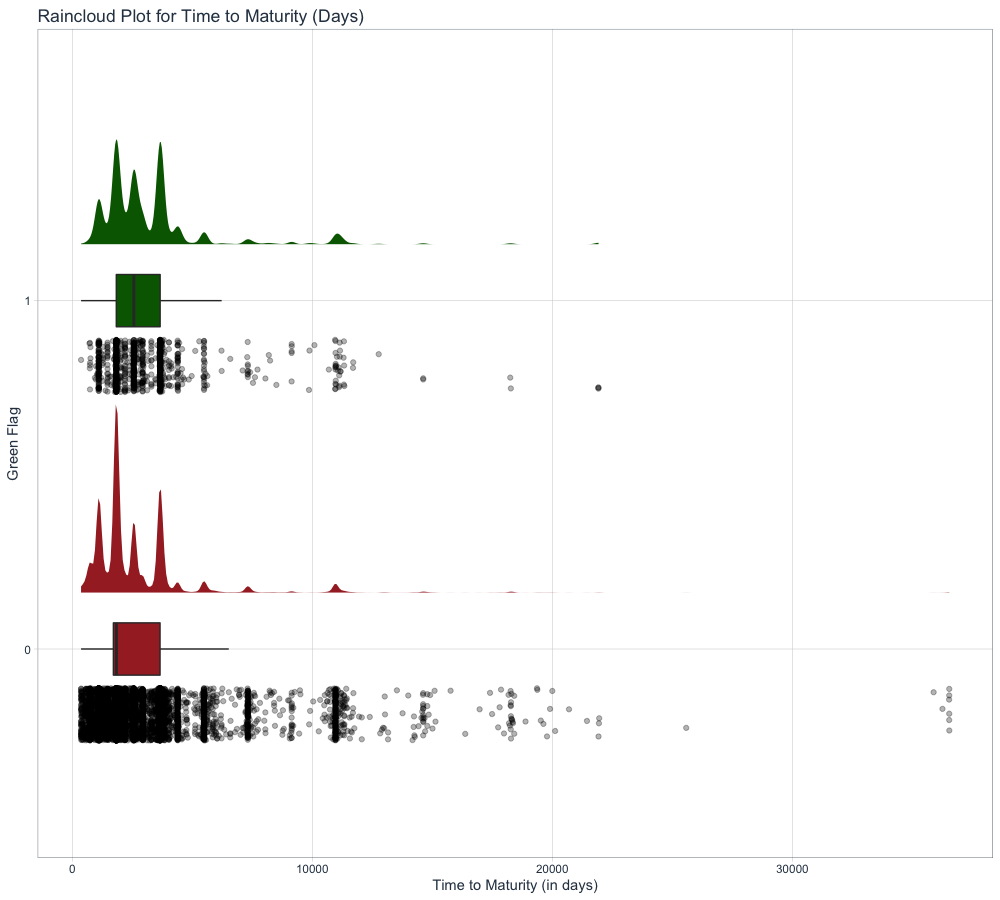
\includegraphics[scale=0.3]{chinchilab-template/chapters/appendices/raincloud_maturity.png}
    \caption{Raincloud Plot for Time to Maturity (Days)}
    \label{rc}
\end{figure}

\begin{figure}[h!]
    \centering
    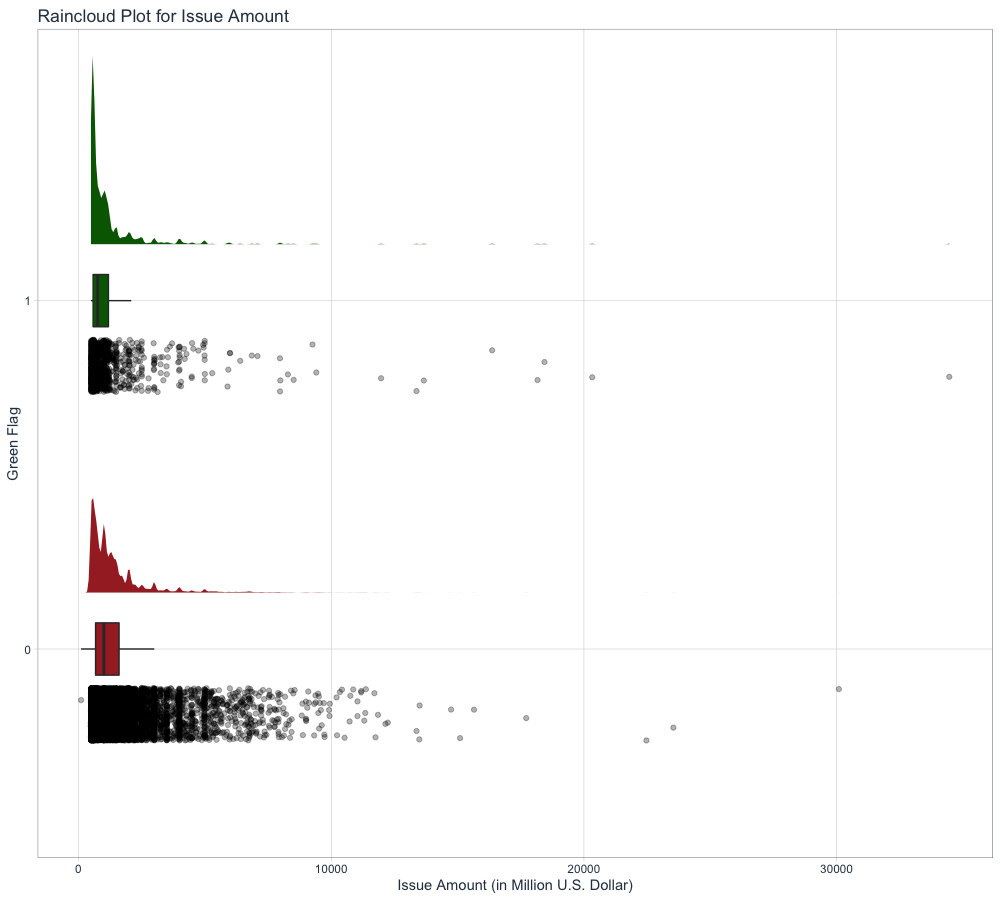
\includegraphics[scale=0.3]{chinchilab-template/chapters/appendices/raincloud_size.png}
    \caption{Raincloud for Issue Amount}
    \label{fig:my_label}
\end{figure}

\begin{figure}[h!]
    \centering
    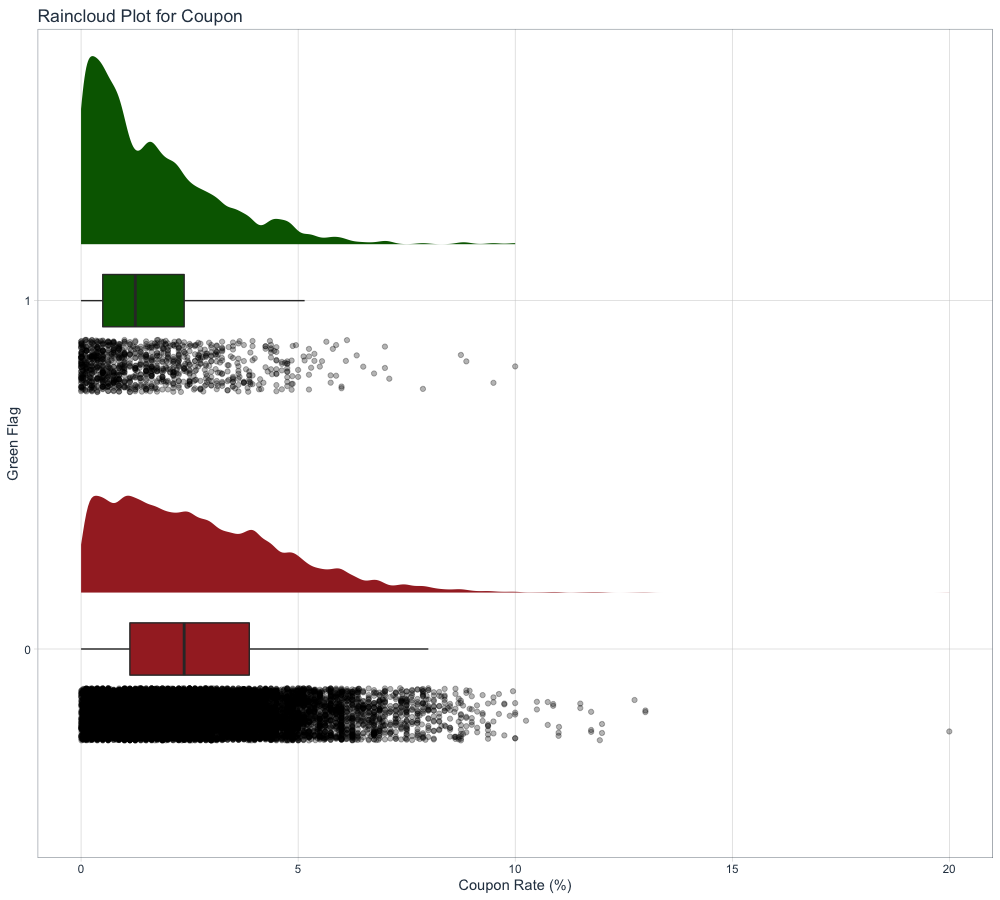
\includegraphics[scale=0.31]{chinchilab-template/chapters/appendices/raincloud_coupon.png}
    \caption{Raincloud for Coupon Rate}
    \label{fig:my_label}
\end{figure}

\begin{figure}[h!]
    \centering
    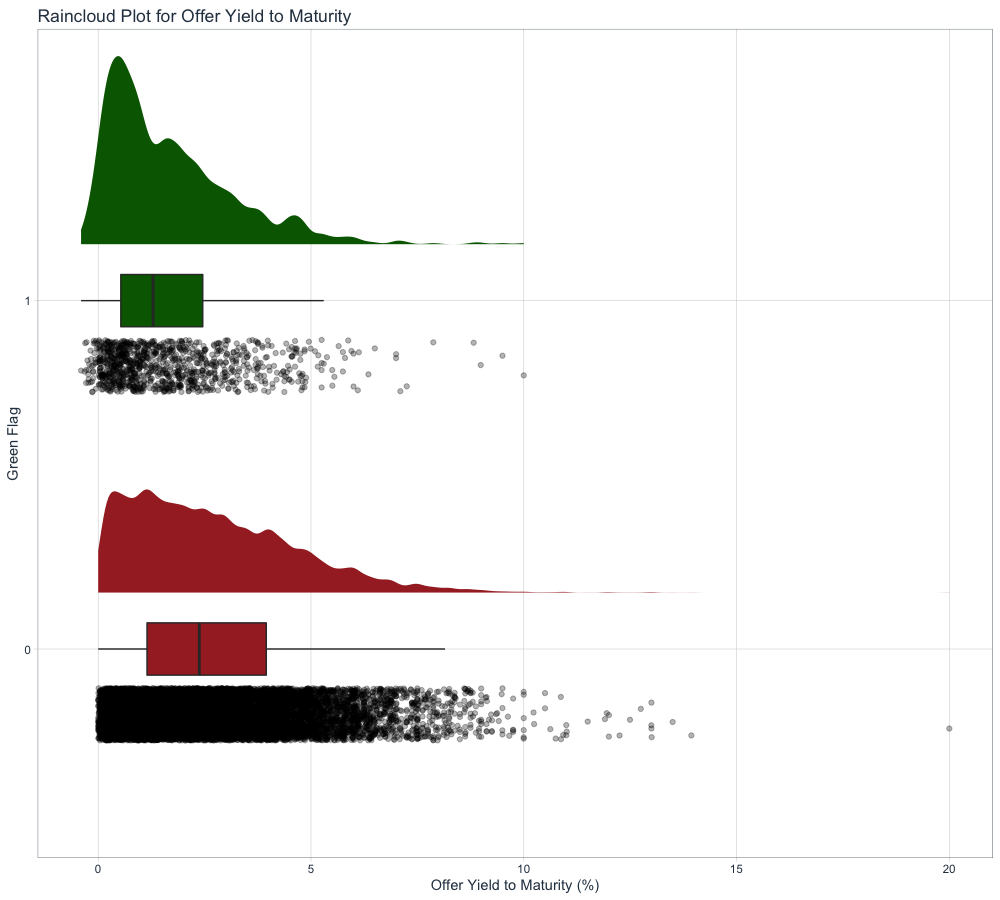
\includegraphics[scale=0.31]{chinchilab-template/chapters/appendices/raincloud_yield.png}
    \caption{Raincloud for Issuance Yield}
    \label{fig:my_label}
\end{figure}

\newpage

\subsection{A.1.3 Propensity Tables}

\begin{table}[h!]
\centering
\caption{Propensity Table for Coupon Frequency}
\label{PROP}
\footnotesize
\begin{tabular}{lll}
\\[-1.8ex]\hline 
\hline \\[-1.8ex] 
\cellcolor[HTML]{FFFFFF}{\color[HTML]{333333} \textbf{Coupon Frequency}} & {\color[HTML]{333333} \textbf{Green (\%)}} & {\color[HTML]{333333} \textbf{Brown (\%)}} \\
\hline \\[-1.8ex] 
{\color[HTML]{333333} Annual Coupon} & \cellcolor[HTML]{006400}{\color[HTML]{FFFFFF} 61.0} & \cellcolor[HTML]{006400}{\color[HTML]{FFFFFF} 58.00} \\
{\color[HTML]{333333} Semi Annual Coupon} & \cellcolor[HTML]{6D9B5F}{\color[HTML]{333333} 38.7} & \cellcolor[HTML]{5A8F4C}{\color[HTML]{FFFFFF} 41.60} \\
{\color[HTML]{333333} Quarterly} & \cellcolor[HTML]{FEFEFE}{\color[HTML]{333333} 0.2} & \cellcolor[HTML]{FEFEFE}{\color[HTML]{333333} 0.20} \\
{\color[HTML]{333333} Monthly} & {\color[HTML]{333333} 0.0} & {\color[HTML]{333333} 0.02} \\
{\color[HTML]{333333} Variable} & {\color[HTML]{333333} 0.0} & {\color[HTML]{333333} 0.01} \\
{\color[HTML]{333333} Maturity} & {\color[HTML]{333333} 0.1} & {\color[HTML]{333333} 0.02} \\
\hline \\[-1.8ex] 
\end{tabular}
\end{table}

\begin{table}[h!] \centering
\caption{Propensity Table for Industry}
\footnotesize
\begin{tabular}{lll}
\\[-1.8ex]\hline 
\hline \\[-1.8ex] 
\cellcolor[HTML]{FFFFFF}{\color[HTML]{333333} \textbf{TRBC Industry}} & \cellcolor[HTML]{FFFFFF}{\color[HTML]{333333} \textbf{Green (\%)}} & \cellcolor[HTML]{FFFFFF}{\color[HTML]{333333} \textbf{Brown (\%)}} \\
\hline \\[-1.8ex] 
{\color[HTML]{333333} Academic \& Educational Services} & \cellcolor[HTML]{FFFFFF}{\color[HTML]{333333} 0.0} & \cellcolor[HTML]{FFFFFF}{\color[HTML]{333333} 0.01} \\
{\color[HTML]{333333} Basic Materials} & \cellcolor[HTML]{F4F8F3}{\color[HTML]{333333} 2.2} & \cellcolor[HTML]{FBFCFA}{\color[HTML]{333333} 1.20} \\
{\color[HTML]{333333} Consumer Cyclicals} & \cellcolor[HTML]{F7F9F6}{\color[HTML]{333333} 1.7} & \cellcolor[HTML]{F9FBF8}{\color[HTML]{333333} 1.70} \\
{\color[HTML]{333333} Consumer Non-Cyclicals} & \cellcolor[HTML]{F8FAF7}{\color[HTML]{333333} 1.5} & \cellcolor[HTML]{FAFCFA}{\color[HTML]{333333} 1.40} \\
{\color[HTML]{333333} Energy} & \cellcolor[HTML]{F9FBF8}{\color[HTML]{333333} 1.3} & \cellcolor[HTML]{FBFCFA}{\color[HTML]{333333} 1.30} \\
{\color[HTML]{333333} Financials} & \cellcolor[HTML]{006400}{\color[HTML]{FFFFFF} 48.4} & \cellcolor[HTML]{006400}{\color[HTML]{FFFFFF} 68.90} \\
{\color[HTML]{333333} Government Activity} & \cellcolor[HTML]{BAD0B2}{\color[HTML]{333333} 14.3} & \cellcolor[HTML]{C5D7BE}{\color[HTML]{333333} 17.10} \\
{\color[HTML]{333333} Healthcare} & \cellcolor[HTML]{FCFDFB}{\color[HTML]{333333} 0.7} & \cellcolor[HTML]{FEFEFE}{\color[HTML]{333333} 0.30} \\
{\color[HTML]{333333} Industrials} & \cellcolor[HTML]{E3ECE0}{\color[HTML]{333333} 5.7} & \cellcolor[HTML]{F7F9F6}{\color[HTML]{333333} 2.40} \\
{\color[HTML]{333333} Institutions, Associations \& Organizations} & \cellcolor[HTML]{E0EADC}{\color[HTML]{333333} 6.4} & \cellcolor[HTML]{F8FAF7}{\color[HTML]{333333} 2.00} \\
{\color[HTML]{333333} Real Estate} & \cellcolor[HTML]{EEF4EC}{\color[HTML]{333333} 3.4} & \cellcolor[HTML]{FEFEFE}{\color[HTML]{333333} 0.30} \\
{\color[HTML]{333333} Technology} & \cellcolor[HTML]{F5F8F3}{\color[HTML]{333333} 2.1} & \cellcolor[HTML]{FAFBF9}{\color[HTML]{333333} 1.60} \\
\cellcolor[HTML]{FFFFFF}{\color[HTML]{333333} Utilities} & \cellcolor[HTML]{C3D6BC}{\color[HTML]{333333} 12.5} & \cellcolor[HTML]{F8FAF7}{\color[HTML]{333333} 2.00} \\
\hline \\[-1.8ex] 
\end{tabular}
\end{table}

\begin{table}[h!] \centering
\caption{Propensity Table for Currency}
\footnotesize
\begin{tabular}{llllll}
\\[-1.8ex]\hline 
\hline \\[-1.8ex] 
\textbf{Currency} & \textbf{Green (\%)} & \textbf{Brown (\%)} &  & \textbf{Green (\%)} & \textbf{Brown (\%)} \\
\hline \\[-1.8ex]
\cellcolor[HTML]{FFFFFF}{\color[HTML]{333333} \textbf{Currency}} & {\color[HTML]{333333} \textbf{Green}} & {\color[HTML]{333333} \textbf{Brown}} & \cellcolor[HTML]{FFFFFF} & {\color[HTML]{333333} \textbf{Green}} & {\color[HTML]{333333} \textbf{Brown}} \\
{\color[HTML]{333333} AUD} & \cellcolor[HTML]{FDFEFD}{\color[HTML]{333333} 0.4} & \cellcolor[HTML]{FBFCFA}{\color[HTML]{333333} 0.90} & {\color[HTML]{333333} NZD} & \cellcolor[HTML]{FEFEFE}{\color[HTML]{333333} 0.2} & {\color[HTML]{333333} 0.10} \\
{\color[HTML]{333333} BRL} & {\color[HTML]{333333} 0.0} & {\color[HTML]{333333} 0.04} & {\color[HTML]{333333} NOK} & {\color[HTML]{333333} 0.1} & {\color[HTML]{333333} 0.04} \\
{\color[HTML]{333333} CAD} & \cellcolor[HTML]{F7F9F5}{\color[HTML]{333333} 2.0} & \cellcolor[HTML]{FBFCFA}{\color[HTML]{333333} 0.90} & {\color[HTML]{333333} PEN} & {\color[HTML]{333333} 0.0} & {\color[HTML]{333333} 0.04} \\
{\color[HTML]{333333} CLP} & {\color[HTML]{333333} 0.1} & {\color[HTML]{333333} 0.02} & {\color[HTML]{333333} PHP} & {\color[HTML]{333333} 0.0} & {\color[HTML]{333333} 0.02} \\
{\color[HTML]{333333} CNY} & {\color[HTML]{333333} 0.1} & {\color[HTML]{333333} 0.04} & {\color[HTML]{333333} RUB} & {\color[HTML]{333333} 0.1} & {\color[HTML]{333333} 0.10} \\
{\color[HTML]{333333} COP} & {\color[HTML]{333333} 0.0} & {\color[HTML]{333333} 0.03} & {\color[HTML]{333333} SGD} & {\color[HTML]{333333} 0.0} & {\color[HTML]{333333} 0.03} \\
{\color[HTML]{333333} HRK} & {\color[HTML]{333333} 0.0} & {\color[HTML]{333333} 0.01} & {\color[HTML]{333333} SEK} & \cellcolor[HTML]{FBFCFB}{\color[HTML]{333333} 0.9} & {\color[HTML]{333333} 0.04} \\
{\color[HTML]{333333} EUR} & \cellcolor[HTML]{006400}{\color[HTML]{FFFFFF} 56.0} & \cellcolor[HTML]{006400}{\color[HTML]{FFFFFF} 48.20} & {\color[HTML]{333333} CHF} & {\color[HTML]{333333} 0.0} & \cellcolor[HTML]{FAFCFA}{\color[HTML]{333333} 1.00} \\
{\color[HTML]{333333} GBP} & \cellcolor[HTML]{F3F7F1}{\color[HTML]{333333} 2.9} & \cellcolor[HTML]{E5EDE1}{\color[HTML]{333333} 5.40} & {\color[HTML]{333333} THB} & {\color[HTML]{333333} 0.0} & {\color[HTML]{333333} 0.03} \\
{\color[HTML]{333333} HKD} & {\color[HTML]{333333} 0.1} & {\color[HTML]{333333} 0.02} & {\color[HTML]{333333} TRY} & {\color[HTML]{333333} 0.0} & {\color[HTML]{333333} 0.02} \\
{\color[HTML]{333333} JPY} & \cellcolor[HTML]{FAFCF9}{\color[HTML]{333333} 1.2} & \cellcolor[HTML]{F0F5EE}{\color[HTML]{333333} 3.10} & {\color[HTML]{333333} USD} & \cellcolor[HTML]{6B9A5E}{\color[HTML]{333333} 35.9} & \cellcolor[HTML]{3F7E32}{\color[HTML]{FFFFFF} 39.90} \\
{\color[HTML]{333333} KZT} & {\color[HTML]{333333} 0.0} & {\color[HTML]{333333} 0.01} & \cellcolor[HTML]{FFFFFF}UYU & \cellcolor[HTML]{FFFFFF}0.1 & \cellcolor[HTML]{FFFFFF}0.03 \\
\cellcolor[HTML]{FFFFFF}{\color[HTML]{333333} MXN} & {\color[HTML]{333333} 0.0} & {\color[HTML]{333333} 0.10} & \cellcolor[HTML]{FFFFFF} & \multicolumn{1}{l}{\cellcolor[HTML]{FFFFFF}} & \multicolumn{1}{l}{\cellcolor[HTML]{FFFFFF}} \\
\hline \\[-1.8ex]
\end{tabular}
\end{table}

\begin{table}[h!] \centering
\caption{Propensity Table for Seniority}
\footnotesize
\begin{tabular}{llllll}
\\[-1.8ex]\hline 
\hline \\[-1.8ex] 
\cellcolor[HTML]{FFFFFF}{\color[HTML]{333333} \textbf{Seniority}} & \cellcolor[HTML]{FFFFFF}{\color[HTML]{333333} \textbf{Green (\%)}} & \cellcolor[HTML]{FFFFFF}{\color[HTML]{333333} \textbf{Brown (\%)}} \\
\hline \\[-1.8ex]
{\color[HTML]{333333} First-Lien Loan} & \cellcolor[HTML]{FEFEFE}{\color[HTML]{333333} 0.3} & \cellcolor[HTML]{FFFFFF}{\color[HTML]{333333} 0.10} \\
{\color[HTML]{333333} First Mortgage} & \cellcolor[HTML]{FAFCFA}{\color[HTML]{333333} 1.4} & \cellcolor[HTML]{FFFFFF}{\color[HTML]{333333} 0.00} \\
{\color[HTML]{333333} First Refunding Mortgage} & \cellcolor[HTML]{FFFFFF}{\color[HTML]{333333} 0.1} & \cellcolor[HTML]{FFFFFF}{\color[HTML]{333333} 0.00} \\
{\color[HTML]{333333} Second-Lien Loan} & \cellcolor[HTML]{FFFFFF}{\color[HTML]{333333} 0.0} & \cellcolor[HTML]{FFFFFF}{\color[HTML]{333333} 0.10} \\
{\color[HTML]{333333} Junior Subordinated} & \cellcolor[HTML]{FEFEFE}{\color[HTML]{333333} 0.3} & \cellcolor[HTML]{FFFFFF}{\color[HTML]{333333} 0.04} \\
{\color[HTML]{333333} Senior Secured Mortgage} & \cellcolor[HTML]{F0F5EE}{\color[HTML]{333333} 4.5} & \cellcolor[HTML]{DFE9DB}{\color[HTML]{333333} 8.40} \\
{\color[HTML]{333333} Refunding Mortgage} & \cellcolor[HTML]{FEFFFE}{\color[HTML]{333333} 0.2} & \cellcolor[HTML]{FDFEFD}{\color[HTML]{333333} 0.40} \\
{\color[HTML]{333333} Senior Secured} & \cellcolor[HTML]{F1F5EF}{\color[HTML]{333333} 4.3} & \cellcolor[HTML]{E2EBDF}{\color[HTML]{333333} 7.60} \\
{\color[HTML]{333333} Senior Unsecured} & \cellcolor[HTML]{006400}{\color[HTML]{FFFFFF} 72.3} & \cellcolor[HTML]{006400}{\color[HTML]{FFFFFF} 62.20} \\
{\color[HTML]{333333} Senior Non-Preferred} & \cellcolor[HTML]{F2F6F1}{\color[HTML]{333333} 3.9} & \cellcolor[HTML]{FAFBF9}{\color[HTML]{333333} 1.40} \\
{\color[HTML]{333333} Senior Preferred} & \cellcolor[HTML]{F0F5EE}{\color[HTML]{333333} 4.7} & \cellcolor[HTML]{F4F8F3}{\color[HTML]{333333} 2.80} \\
{\color[HTML]{333333} Senior Subordinated Unsecured} & \cellcolor[HTML]{FFFFFF}{\color[HTML]{333333} 0.1} & \cellcolor[HTML]{FDFEFD}{\color[HTML]{333333} 0.50} \\
{\color[HTML]{333333} Senior Subordinated Secured} & \cellcolor[HTML]{FFFFFF}{\color[HTML]{333333} 0.0} & \cellcolor[HTML]{FFFFFF}{\color[HTML]{333333} 0.01} \\
{\color[HTML]{333333} Subordinated Unsecured} & \cellcolor[HTML]{FDFEFD}{\color[HTML]{333333} 0.5} & \cellcolor[HTML]{F7FAF6}{\color[HTML]{333333} 2.00} \\
{\color[HTML]{333333} Subordinated Secured} & \cellcolor[HTML]{FFFFFF}{\color[HTML]{333333} 0.0} & \cellcolor[HTML]{FFFFFF}{\color[HTML]{333333} 0.01} \\
{\color[HTML]{333333} Unsecured} & \cellcolor[HTML]{F7FAF7}{\color[HTML]{333333} 2.3} & \cellcolor[HTML]{D6E3D1}{\color[HTML]{333333} 10.80} \\
\hline \\[-1.8ex]
\end{tabular}
\end{table}




\begin{table}[H]{
    \begin{subtable}{.5\textwidth}
    \centering
    \footnotesize
        {\begin{tabular}{lll}
        \\[-1.8ex]\hline 
        \hline \\[-1.8ex] 
        \textbf{Issuer Sector} & \textbf{Green (\%)} & \textbf{Brown (\%)} \\
        \hline \\[-1.8ex]
        \cellcolor[HTML]{FFFFFF}{\color[HTML]{333333} Public Sector} & {\color[HTML]{333333} 36.2} & {\color[HTML]{333333} 38.2} \\
        \rowcolor[HTML]{006400} 
        \cellcolor[HTML]{FFFFFF}{\color[HTML]{333333} Corporate Sector} & {\color[HTML]{FFFFFF} 63.8} & {\color[HTML]{FFFFFF} 61.8} \\
        \\[-1.8ex]\hline 
        \end{tabular}}
    \subcaption{Issuer Sector}
    \end{subtable}
    \begin{subtable}{0.3\linewidth}
    \centering
    \footnotesize
        {\begin{tabular}{lll}
        \\[-1.8ex]\hline 
        \hline \\[-1.8ex] 
        \textbf{Guarantor} & \textbf{Green (\%)} & \textbf{Brown (\%)} \\
        \hline \\[-1.8ex]
        \rowcolor[HTML]{FFFFFF} 
        {\color[HTML]{333333} Guarantor} & {\color[HTML]{333333} 18.4} & {\color[HTML]{333333} 24} \\
        \rowcolor[HTML]{006400} 
        \cellcolor[HTML]{FAFAFA}{\color[HTML]{333333} No Guarantor} & {\color[HTML]{FFFFFF} 81.6} & {\color[HTML]{FFFFFF} 76} \\
        \hline \\[-1.8ex]
        \end{tabular}}
    \subcaption{Guarantor}
    \end{subtable}
\caption{Propensity Table for Issuer Sector and Guarantor}
\label{x}}
\end{table}

%%%%%%%%%%%%%%%%%%%%%%%%%%%%%%%%%%%%%%%%%%%%%%%%%%%%%%%%%%%%
\section{A.2 Causal Forest}
%%%%%%%%%%%%%%%%%%%%%%%%%%%%%%%%%%%%%%%%%%%%%%%%%%%%%%%%%%%%

%%%%%%%%%%%%%%%%%%%%%%%%%%%%%%%%%%%%%%%%%%%%%%%%%%%%%%%%%%%%
\subsection{A.2.1 Without Issuer Controls}
%%%%%%%%%%%%%%%%%%%%%%%%%%%%%%%%%%%%%%%%%%%%%%%%%%%%%%%%%%%%

\begin{figure}[H]
    \centering
    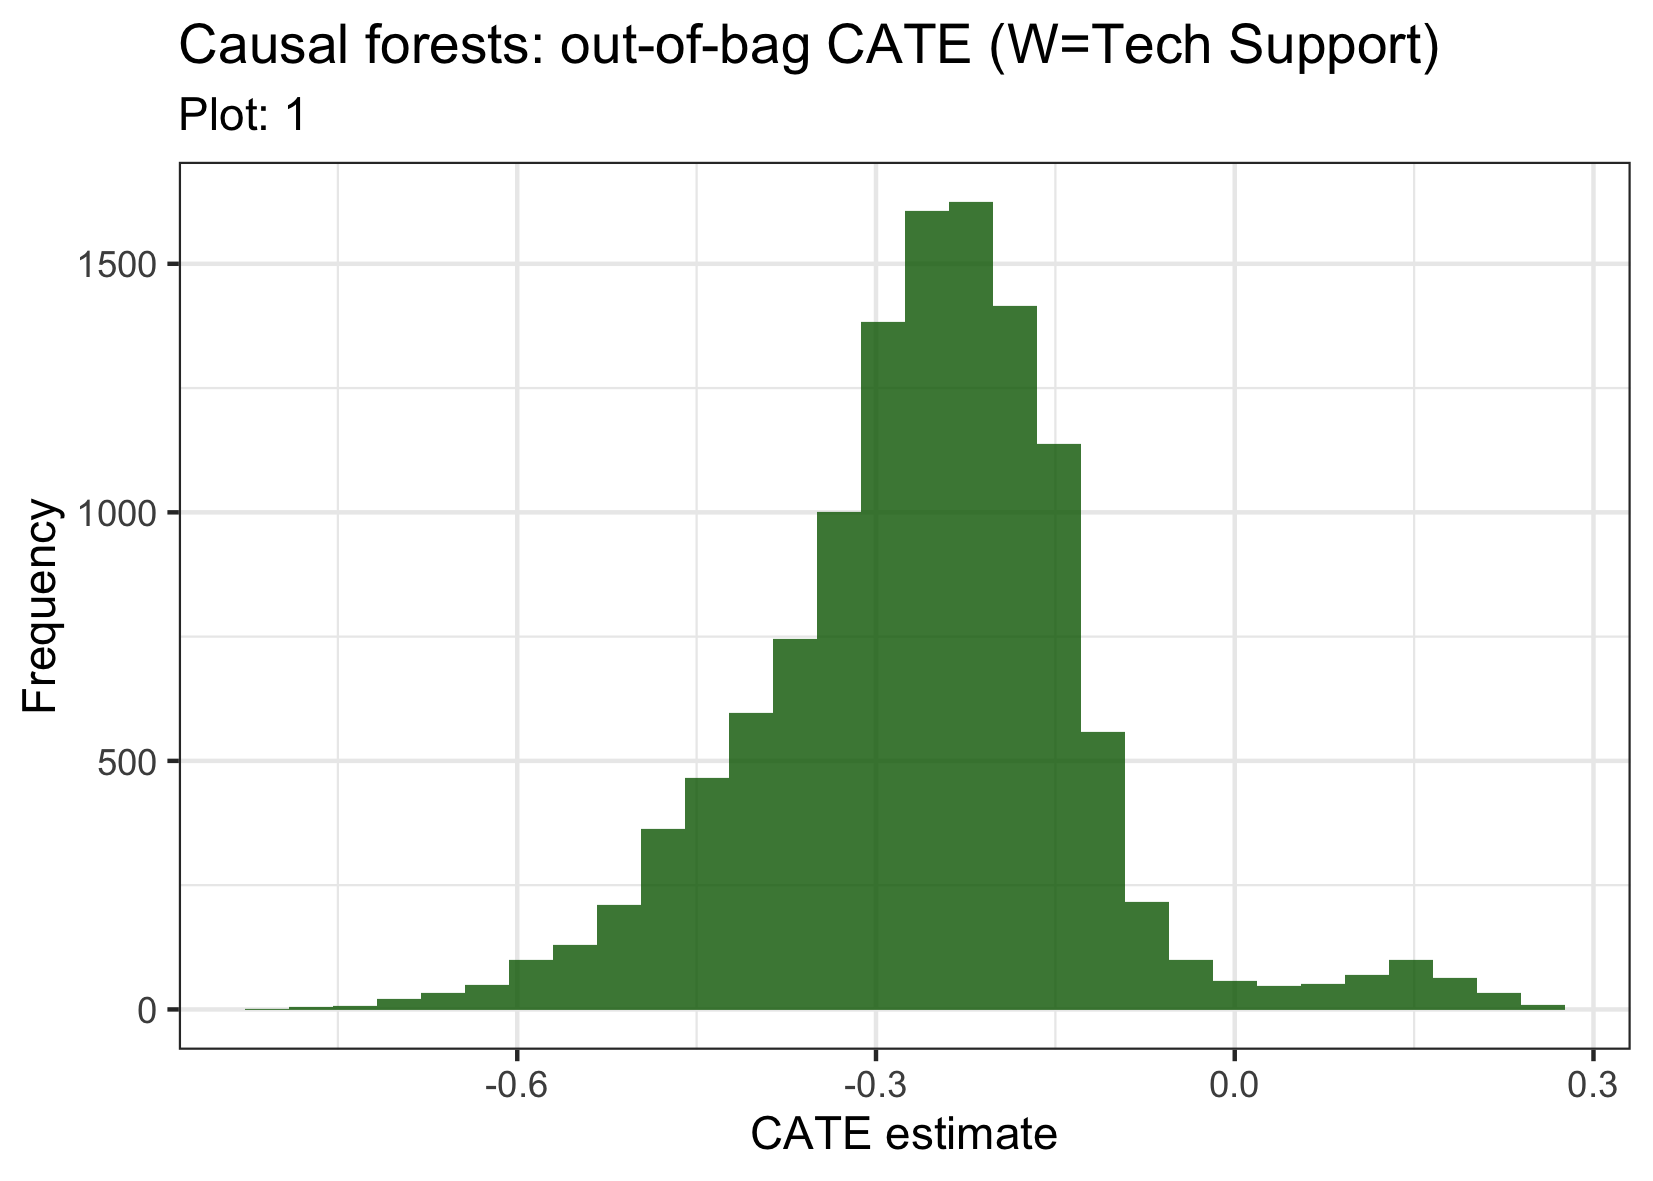
\includegraphics[scale=0.15]{chinchilab-template/chapters/appendices/ANALYSIS/CATE_1.png}
    \caption{Distribution of CATE (Model 1)}
    \label{fig:my_label}
\end{figure}

%%%%%%%%%%%%%%%%%%%%%%%%%%%%%%%%%%%%%%%%%%%%%%%%%%%%%%%%%%%%
\subsubsection{A.2.1.1 Nuisance Parameter Check}
%%%%%%%%%%%%%%%%%%%%%%%%%%%%%%%%%%%%%%%%%%%%%%%%%%%%%%%%%%%%
\begin{figure}[h!]
    \centering
    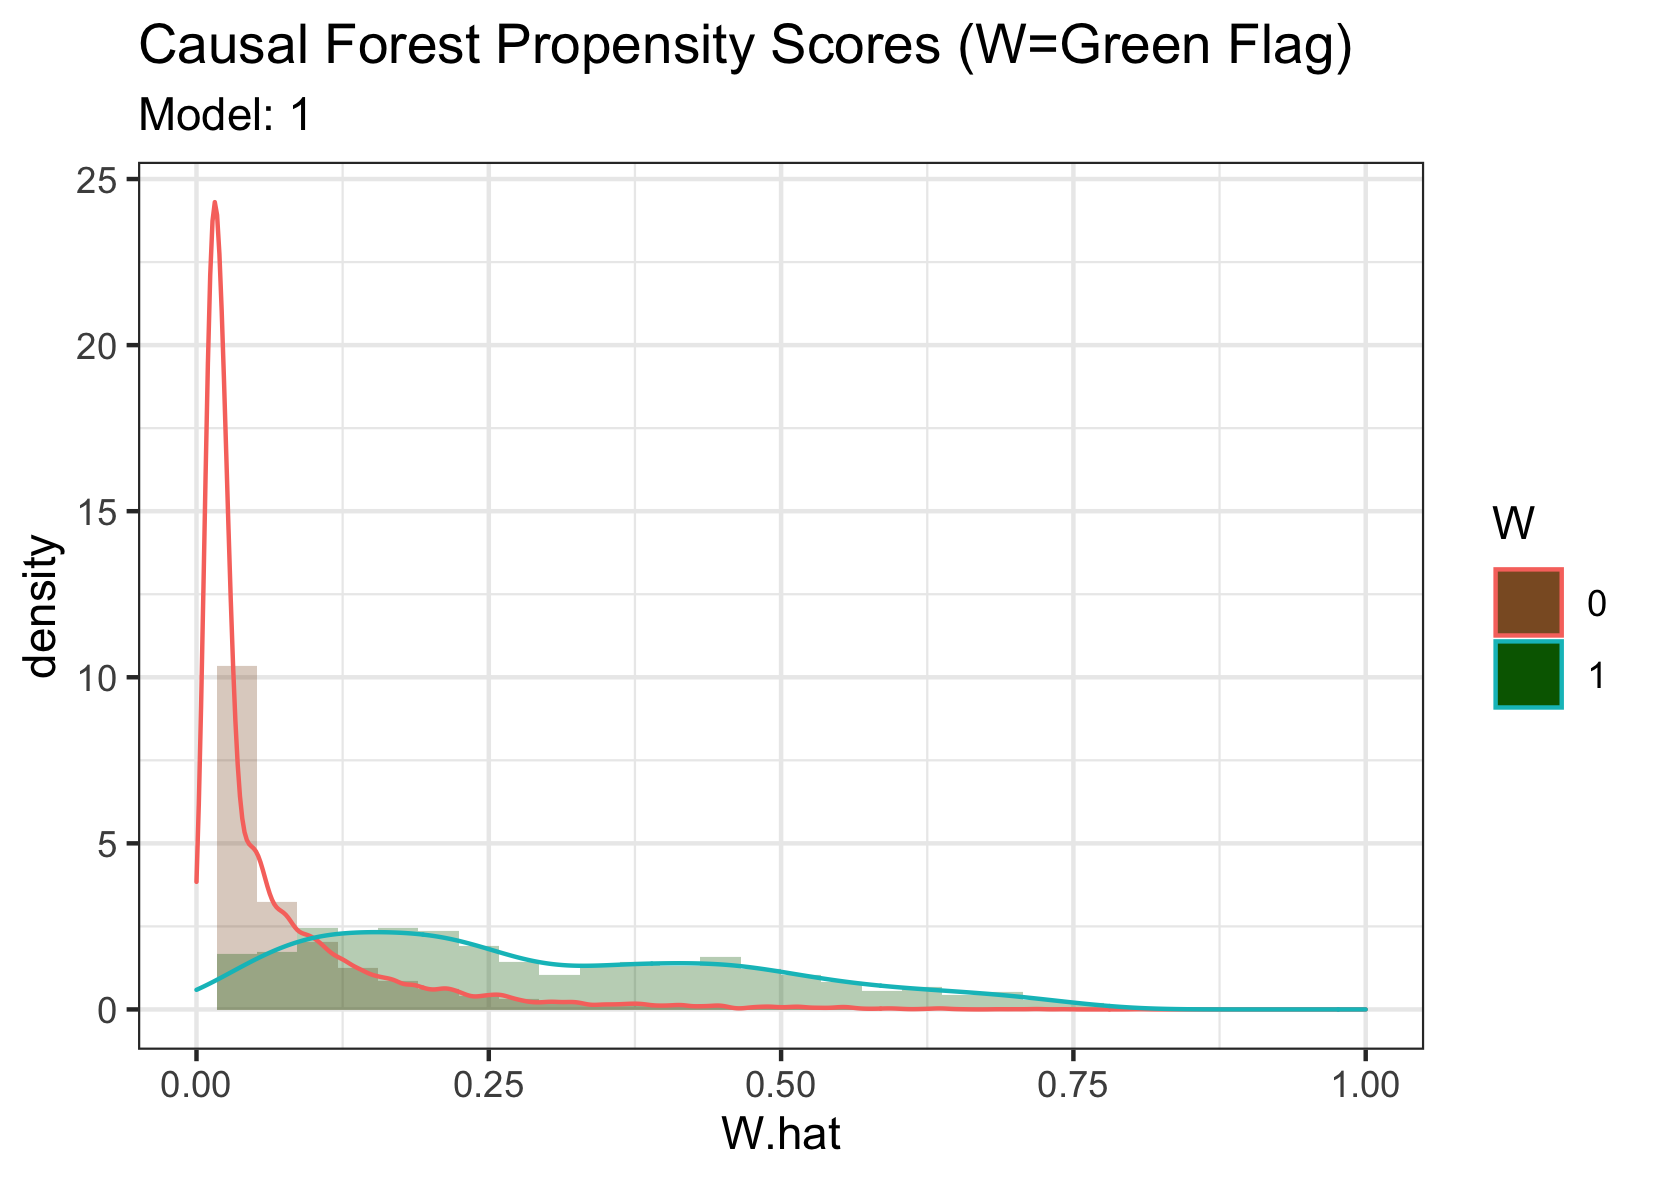
\includegraphics[scale=0.17]{chinchilab-template/chapters/appendices/ANALYSIS/prop_1.png}
    \caption{Propensity Score Distribution (Model 1)}
    \label{fig:my_label}
\end{figure}

\begin{table}[H]{
    \begin{subtable}{.5\textwidth}
    \centering
    \footnotesize
        {\begin{tabular}{@{\extracolsep{5pt}}lc} 
        \\[-1.8ex]\hline 
        \hline \\[-1.8ex] 
         & \multicolumn{1}{c}{\textit{Dependent variable: Green Flag}} \\ 
        \cline{2-2} 
        \\[-1.8ex] &   \\ 
        \hline \\[-1.8ex] 
         e.bar & 1.008$^{***}$ \\ 
          & (0.025) \\ 
          & \\ 
         e.residual & 1.254$^{***}$ \\ 
          & (0.032) \\ 
          & \\ 
        \hline \\[-1.8ex] 
        \hline 
        \hline \\[-1.8ex] 
        \textit{Note:}  & \multicolumn{1}{r}{$^{*}$p$<$0.1; $^{**}$p$<$0.05; $^{***}$p$<$0.01} \\ 
        \end{tabular} }
    \subcaption{Outcome Model}
    \end{subtable}
    \begin{subtable}{0.3\linewidth}
    \centering
    \footnotesize
        {\begin{tabular}{@{\extracolsep{5pt}}lc} 
        \\[-1.8ex]\hline 
        \hline \\[-1.8ex] 
         & \multicolumn{1}{c}{\textit{Dependent variable: Green Flag}} \\ 
        \cline{2-2} 
        \\[-1.8ex] &   \\ 
        \hline \\[-1.8ex] 
         m.bar & 0.999$^{***}$ \\ 
          & (0.003) \\ 
          & \\ 
         m.residual & 1.173$^{***}$ \\ 
          & (0.008) \\ 
          & \\ 
        \hline \\[-1.8ex] 
        \hline 
        \hline \\[-1.8ex] 
        \textit{Note:}  & \multicolumn{1}{r}{$^{*}$p$<$0.1; $^{**}$p$<$0.05; $^{***}$p$<$0.01} \\ 
        \end{tabular} }
    \subcaption{Propensity Model}
    \end{subtable}
\caption{Calibration Regressions (Model 1)}
\label{x}}
\end{table}

%%%%%%%%%%%%%%%%%%%%%%%%%%%%%%%%%%%%%%%%%%%%%%%%%%%%%%%%%%%%
\subsubsection{A.2.1.2 Heterogeneity Assessment}
%%%%%%%%%%%%%%%%%%%%%%%%%%%%%%%%%%%%%%%%%%%%%%%%%%%%%%%%%%%%

\begin{table}[h!]
\centering
\caption{Variable Importance (Model 1)}
\begin{tabular}{lr}
\\[-1.8ex]\hline 
\hline \\[-1.8ex] 
\rowcolor[HTML]{FFFFFF} 
{\color[HTML]{333333} \textbf{Covariate}} & {\color[HTML]{333333} \textbf{Value}} \\ \hline
\rowcolor[HTML]{FFFFFF} 
{\color[HTML]{333333} 2022} & \cellcolor[HTML]{00441B}{\color[HTML]{FFFFFF} 0.18699691} \\
\rowcolor[HTML]{FFFFFF} 
{\color[HTML]{333333} Issue Amount} & \cellcolor[HTML]{288F48}{\color[HTML]{FFFFFF} 0.15014007} \\
\rowcolor[HTML]{FFFFFF} 
{\color[HTML]{333333} Utilities} & \cellcolor[HTML]{77C578}{\color[HTML]{333333} 0.11702269} \\
\rowcolor[HTML]{FFFFFF} 
{\color[HTML]{333333} Time to Maturity (Days)} & \cellcolor[HTML]{78C679}{\color[HTML]{333333} 0.11682995} \\
\rowcolor[HTML]{FFFFFF} 
{\color[HTML]{333333} BBB} & \cellcolor[HTML]{F5FBF3}{\color[HTML]{333333} 0.05125039} \\
\rowcolor[HTML]{FFFFFF} 
{\color[HTML]{333333} Financials} & \cellcolor[HTML]{F7FCF5}{\color[HTML]{333333} 0.04937156} \\ \hline
\end{tabular}
\end{table}

\newpage

\begin{figure}[h!]
    \centering
    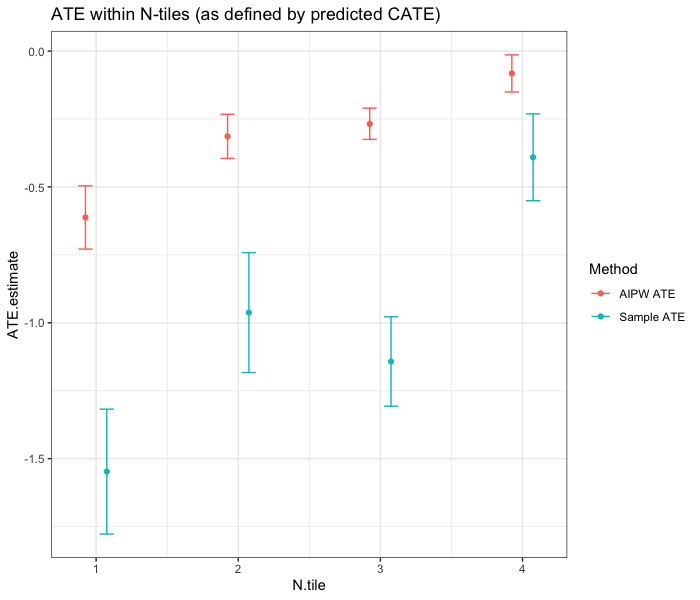
\includegraphics[scale=0.35]{chinchilab-template/chapters/appendices/ANALYSIS/ntile_cf0.png}
    \caption{Graph of ATE within Subgroups (Model 1)}
    \label{fig:my_label}
\end{figure}



\begin{figure}[H]
\centering
   \begin{subfigure}[b]{0.45\textwidth}
    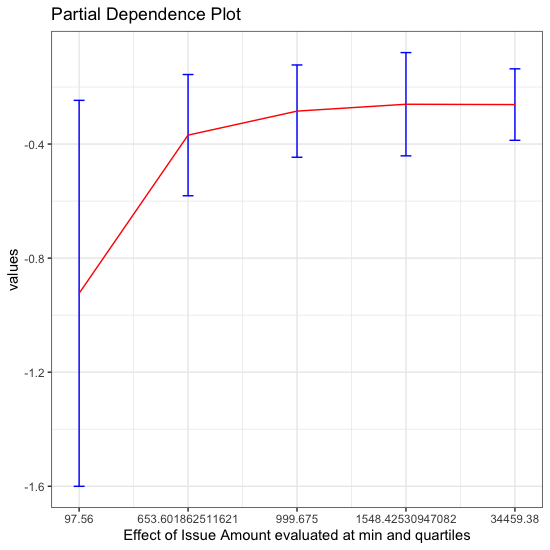
\includegraphics[width=0.8\textwidth]{chinchilab-template/chapters/appendices/ANALYSIS/PDP_cf0.png}
    \caption{Effect of Issue Amount}
   \label{fig:Ng1} 
\end{subfigure}
\begin{subfigure}[b]{0.45\textwidth}
    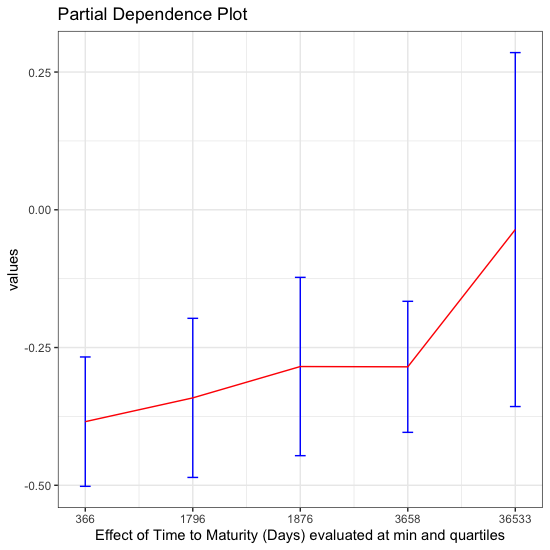
\includegraphics[width=0.8\textwidth]{chinchilab-template/chapters/appendices/ANALYSIS/PDP2_cf0.png}
    \caption{Effect of Time to Maturity (Days)}
   \label{fig:Ng2}
\end{subfigure}
\\
\begin{subfigure}[b]{0.45\textwidth}
    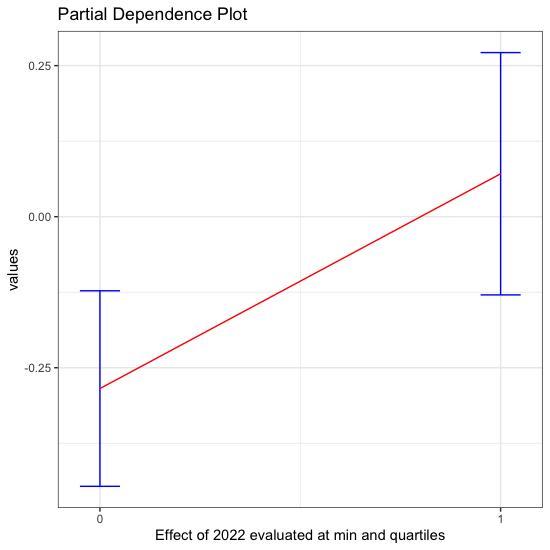
\includegraphics[width=0.8\textwidth]{chinchilab-template/chapters/appendices/ANALYSIS/PDP3_cf0.png}
    \caption{Effect of 2022}
   \label{fig:Ng2}
\end{subfigure}
\caption{Partial Dependence Plots (Model 1)}
\end{figure}


\begin{table}[h!]
\caption{Heterogeneity across Covariates (Model 1)}
\label{Het}
\footnotesize
\begin{tabular}{lllll}
\\[-1.8ex]\hline 
\hline \\[-1.8ex] 
{\color[HTML]{333333} \textbf{Variable}} & {\color[HTML]{333333} \textbf{Mean ntile1}} & {\color[HTML]{333333} \textbf{Mean ntile2}} & {\color[HTML]{333333} \textbf{Mean ntile3}} & {\color[HTML]{333333} \textbf{Mean ntile4}} \\
\hline \\[-1.8ex] 
\cellcolor[HTML]{FFFFFF}Time to   Maturity (Days) & \cellcolor[HTML]{63BE7B}2882.61 & \cellcolor[HTML]{E6F3EC}2628.35 & \cellcolor[HTML]{FCFCFF}2585.12 & \cellcolor[HTML]{8BCF9E}2805.31 \\
\cellcolor[HTML]{FFFFFF}Issue Amount & \cellcolor[HTML]{FCFCFF}974.29 & \cellcolor[HTML]{CCE9D5}1274.77 & \cellcolor[HTML]{94D2A5}1618.74 & \cellcolor[HTML]{63BE7B}1916.95 \\
\cellcolor[HTML]{FFFFFF}Guarantor & \cellcolor[HTML]{D1EBDA}0.25 & \cellcolor[HTML]{D6EDDE}0.22 & \cellcolor[HTML]{D8EEE0}0.21 & \cellcolor[HTML]{CDE9D7}0.27 \\
\cellcolor[HTML]{FFFFFF}2013 & \cellcolor[HTML]{E9F5EF}0.11 & \cellcolor[HTML]{F0F8F5}0.07 & \cellcolor[HTML]{F0F8F5}0.07 & \cellcolor[HTML]{F5FAF9}0.04 \\
\cellcolor[HTML]{FFFFFF}2014 & \cellcolor[HTML]{EDF6F2}0.09 & \cellcolor[HTML]{EEF7F3}0.08 & \cellcolor[HTML]{F2F8F6}0.06 & \cellcolor[HTML]{F4F9F8}0.05 \\
\cellcolor[HTML]{FFFFFF}2015 & \cellcolor[HTML]{F0F8F5}0.07 & \cellcolor[HTML]{EEF7F3}0.08 & \cellcolor[HTML]{F0F8F5}0.07 & \cellcolor[HTML]{F2F8F6}0.06 \\
\cellcolor[HTML]{FFFFFF}2016 & \cellcolor[HTML]{F0F8F5}0.07 & \cellcolor[HTML]{EEF7F3}0.08 & \cellcolor[HTML]{F2F8F6}0.06 & \cellcolor[HTML]{F4F9F8}0.05 \\
\cellcolor[HTML]{FFFFFF}2017 & \cellcolor[HTML]{F2F8F6}0.06 & \cellcolor[HTML]{EEF7F3}0.08 & \cellcolor[HTML]{F0F8F5}0.07 & \cellcolor[HTML]{F5FAF9}0.04 \\
\cellcolor[HTML]{FFFFFF}2018 & \cellcolor[HTML]{F9FBFC}0.02 & \cellcolor[HTML]{F7FAFB}0.03 & \cellcolor[HTML]{EDF6F2}0.09 & \cellcolor[HTML]{EDF6F2}0.09 \\
\cellcolor[HTML]{FFFFFF}2019 & \cellcolor[HTML]{F2F8F6}0.06 & \cellcolor[HTML]{E9F5EF}0.11 & \cellcolor[HTML]{EEF7F3}0.08 & \cellcolor[HTML]{F9FBFC}0.02 \\
\cellcolor[HTML]{FFFFFF}2020 & \cellcolor[HTML]{F9FBFC}0.02 & \cellcolor[HTML]{F9FBFC}0.02 & \cellcolor[HTML]{F4F9F8}0.05 & \cellcolor[HTML]{E4F3EA}0.14 \\
\cellcolor[HTML]{FFFFFF}2021 & \cellcolor[HTML]{F7FAFB}0.03 & \cellcolor[HTML]{F4F9F8}0.05 & \cellcolor[HTML]{EDF6F2}0.09 & \cellcolor[HTML]{F0F8F5}0.07 \\
\cellcolor[HTML]{FFFFFF}2022 & \cellcolor[HTML]{FCFCFF}0 & \cellcolor[HTML]{FBFCFE}0.01 & \cellcolor[HTML]{FBFCFE}0.01 & \cellcolor[HTML]{DFF0E6}0.17 \\
\cellcolor[HTML]{FFFFFF}Annual Coupon & \cellcolor[HTML]{A3D8B2}0.51 & \cellcolor[HTML]{81CB95}0.7 & \cellcolor[HTML]{87CD9A}0.67 & \cellcolor[HTML]{A8DAB7}0.48 \\
\cellcolor[HTML]{FFFFFF}Semi Annual   Coupon & \cellcolor[HTML]{A6DAB5}0.49 & \cellcolor[HTML]{C8E7D2}0.3 & \cellcolor[HTML]{C2E5CD}0.33 & \cellcolor[HTML]{A1D7B1}0.52 \\
\rowcolor[HTML]{FCFCFF} 
\cellcolor[HTML]{FFFFFF}Quarterly & 0 & 0 & 0 & 0 \\
\rowcolor[HTML]{FCFCFF} 
\cellcolor[HTML]{FFFFFF}Monthly & 0 & 0 & 0 & 0 \\
\rowcolor[HTML]{FCFCFF} 
\cellcolor[HTML]{FFFFFF}Variable & 0 & 0 & 0 & 0 \\
\rowcolor[HTML]{FCFCFF} 
\cellcolor[HTML]{FFFFFF}First Lien Loan & 0 & 0 & 0 & 0 \\
\rowcolor[HTML]{FCFCFF} 
\cellcolor[HTML]{FFFFFF}First Mortgage & 0 & 0 & 0 & 0 \\
\rowcolor[HTML]{FCFCFF} 
\cellcolor[HTML]{FFFFFF}First   Refunding Mortgage & 0 & 0 & 0 & 0 \\
\rowcolor[HTML]{FCFCFF} 
\cellcolor[HTML]{FFFFFF}Second Lien Loan & 0 & 0 & 0 & 0 \\
\rowcolor[HTML]{FCFCFF} 
\cellcolor[HTML]{FFFFFF}Junior   Subordinated & 0 & 0 & 0 & 0 \\
\cellcolor[HTML]{FFFFFF}Senior   Secured Mortgage & \cellcolor[HTML]{FCFCFF}0 & \cellcolor[HTML]{E9F5EF}0.11 & \cellcolor[HTML]{E6F3EC}0.13 & \cellcolor[HTML]{EDF6F2}0.09 \\
\rowcolor[HTML]{FCFCFF} 
\cellcolor[HTML]{FFFFFF}Refunding   Mortgage & 0 & 0 & \cellcolor[HTML]{FBFCFE}0.01 & 0 \\
\cellcolor[HTML]{FFFFFF}Senior Secured & \cellcolor[HTML]{F9FBFC}0.02 & \cellcolor[HTML]{F0F8F5}0.07 & \cellcolor[HTML]{EBF5F0}0.1 & \cellcolor[HTML]{E7F4ED}0.12 \\
\cellcolor[HTML]{FFFFFF}Senior Unsecured & \cellcolor[HTML]{63BE7B}0.87 & \cellcolor[HTML]{88CD9B}0.66 & \cellcolor[HTML]{9ED6AE}0.54 & \cellcolor[HTML]{A1D7B1}0.52 \\
\cellcolor[HTML]{FFFFFF}Senior Non   Preferred & \cellcolor[HTML]{FCFCFF}0 & \cellcolor[HTML]{FBFCFE}0.01 & \cellcolor[HTML]{F9FBFC}0.02 & \cellcolor[HTML]{F5FAF9}0.04 \\
\cellcolor[HTML]{FFFFFF}Senior Preferred & \cellcolor[HTML]{FCFCFF}0 & \cellcolor[HTML]{FBFCFE}0.01 & \cellcolor[HTML]{F4F9F8}0.05 & \cellcolor[HTML]{F2F8F6}0.06 \\
\cellcolor[HTML]{FFFFFF}Senior   Subordinated Unsecured & \cellcolor[HTML]{FBFCFE}0.01 & \cellcolor[HTML]{FCFCFF}0 & \cellcolor[HTML]{FBFCFE}0.01 & \cellcolor[HTML]{FCFCFF}0 \\
\rowcolor[HTML]{FCFCFF} 
\cellcolor[HTML]{FFFFFF}Senior   Subordinated Secured & 0 & 0 & 0 & 0 \\
\cellcolor[HTML]{FFFFFF}Subordinated   Unsecured & \cellcolor[HTML]{F7FAFB}0.03 & \cellcolor[HTML]{F9FBFC}0.02 & \cellcolor[HTML]{F9FBFC}0.02 & \cellcolor[HTML]{FBFCFE}0.01 \\
\rowcolor[HTML]{FCFCFF} 
\cellcolor[HTML]{FFFFFF}Subordinated   Secured & 0 & 0 & 0 & 0 \\
\rowcolor[HTML]{FCFCFF} 
\cellcolor[HTML]{FFFFFF}Academic   \& Educational Services & 0 & 0 & 0 & 0 \\
\cellcolor[HTML]{FFFFFF}Basic Materials & \cellcolor[HTML]{F5FAF9}0.04 & \cellcolor[HTML]{FBFCFE}0.01 & \cellcolor[HTML]{FCFCFF}0 & \cellcolor[HTML]{FCFCFF}0 \\
\cellcolor[HTML]{FFFFFF}Consumer   Cyclicals & \cellcolor[HTML]{F5FAF9}0.04 & \cellcolor[HTML]{F9FBFC}0.02 & \cellcolor[HTML]{FBFCFE}0.01 & \cellcolor[HTML]{FCFCFF}0 \\
\cellcolor[HTML]{FFFFFF}Consumer   Non Cyclicals & \cellcolor[HTML]{F5FAF9}0.04 & \cellcolor[HTML]{FBFCFE}0.01 & \cellcolor[HTML]{FBFCFE}0.01 & \cellcolor[HTML]{FCFCFF}0 \\
\cellcolor[HTML]{FFFFFF}Energy & \cellcolor[HTML]{F5FAF9}0.04 & \cellcolor[HTML]{FBFCFE}0.01 & \cellcolor[HTML]{FCFCFF}0 & \cellcolor[HTML]{FCFCFF}0 \\
\cellcolor[HTML]{FFFFFF}Financials & \cellcolor[HTML]{ADDCBB}0.45 & \cellcolor[HTML]{8ACE9D}0.65 & \cellcolor[HTML]{7AC88F}0.74 & \cellcolor[HTML]{69C180}0.84 \\
\rowcolor[HTML]{FCFCFF} 
\cellcolor[HTML]{FFFFFF}Healthcare & \cellcolor[HTML]{FBFCFE}0.01 & 0 & 0 & 0 \\
\cellcolor[HTML]{FFFFFF}Industrials & \cellcolor[HTML]{F2F8F6}0.06 & \cellcolor[HTML]{F7FAFB}0.03 & \cellcolor[HTML]{FBFCFE}0.01 & \cellcolor[HTML]{FBFCFE}0.01 \\
\cellcolor[HTML]{FFFFFF}Institutions,   Associations \& Organizations & \cellcolor[HTML]{FCFCFF}0 & \cellcolor[HTML]{F9FBFC}0.02 & \cellcolor[HTML]{F4F9F8}0.05 & \cellcolor[HTML]{F7FAFB}0.03 \\
\cellcolor[HTML]{FFFFFF}Real Estate & \cellcolor[HTML]{FBFCFE}0.01 & \cellcolor[HTML]{FBFCFE}0.01 & \cellcolor[HTML]{FCFCFF}0 & \cellcolor[HTML]{FCFCFF}0 \\
\cellcolor[HTML]{FFFFFF}Technology & \cellcolor[HTML]{F4F9F8}0.05 & \cellcolor[HTML]{FBFCFE}0.01 & \cellcolor[HTML]{FBFCFE}0.01 & \cellcolor[HTML]{FCFCFF}0 \\
\rowcolor[HTML]{FCFCFF} 
\cellcolor[HTML]{FFFFFF}Utilities & \cellcolor[HTML]{E9F5EF}0.11 & 0 & 0 & 0 \\
\cellcolor[HTML]{FFFFFF}AAA & \cellcolor[HTML]{F0F8F5}0.07 & \cellcolor[HTML]{C4E6CF}0.32 & \cellcolor[HTML]{A5D9B4}0.5 & \cellcolor[HTML]{A1D7B1}0.52 \\
\cellcolor[HTML]{FFFFFF}AA & \cellcolor[HTML]{F0F8F5}0.07 & \cellcolor[HTML]{D4ECDD}0.23 & \cellcolor[HTML]{CDE9D7}0.27 & \cellcolor[HTML]{C6E6D0}0.31 \\
\cellcolor[HTML]{FFFFFF}A & \cellcolor[HTML]{C6E6D0}0.31 & \cellcolor[HTML]{CFEAD8}0.26 & \cellcolor[HTML]{E6F3EC}0.13 & \cellcolor[HTML]{EEF7F3}0.08 \\
\cellcolor[HTML]{FFFFFF}BBB & \cellcolor[HTML]{B3DFC0}0.42 & \cellcolor[HTML]{E7F4ED}0.12 & \cellcolor[HTML]{F0F8F5}0.07 & \cellcolor[HTML]{F0F8F5}0.07 \\
\cellcolor[HTML]{FFFFFF}BB & \cellcolor[HTML]{EEF7F3}0.08 & \cellcolor[HTML]{F4F9F8}0.05 & \cellcolor[HTML]{F9FBFC}0.02 & \cellcolor[HTML]{FBFCFE}0.01 \\
\cellcolor[HTML]{FFFFFF}B & \cellcolor[HTML]{F4F9F8}0.05 & \cellcolor[HTML]{F9FBFC}0.02 & \cellcolor[HTML]{FBFCFE}0.01 & \cellcolor[HTML]{FCFCFF}0 \\
\hline \\[-1.8ex] 
\end{tabular}
\end{table}

\begin{table}[H]
\centering
\caption{Heterogeneity across Covariates cont. (Model 1)}
\label{Het}
\footnotesize
\begin{tabular}{lllll}
\\[-1.8ex]\hline 
\hline \\[-1.8ex] 
{\color[HTML]{333333} \textbf{Variable}} & {\color[HTML]{333333} \textbf{Mean ntile1}} & {\color[HTML]{333333} \textbf{Mean ntile2}} & {\color[HTML]{333333} \textbf{Mean ntile3}} & {\color[HTML]{333333} \textbf{Mean ntile4}} \\
\hline \\[-1.8ex] 
AUD & 0 & \cellcolor[HTML]{FBFCFE}0.01 & \cellcolor[HTML]{FBFCFE}0.01 & \cellcolor[HTML]{FBFCFE}0.01 \\
BRL & 0 & 0 & 0 & 0 \\
EUR & \cellcolor[HTML]{B3DFC0}0.42 & \cellcolor[HTML]{91D1A3}0.61 & \cellcolor[HTML]{9AD5AB}0.56 & \cellcolor[HTML]{BAE1C6}0.38 \\
GBP & \cellcolor[HTML]{F4F9F8}0.05 & \cellcolor[HTML]{F7FAFB}0.03 & \cellcolor[HTML]{F4F9F8}0.05 & \cellcolor[HTML]{EEF7F3}0.08 \\
HKD & 0 & 0 & 0 & 0 \\
JPY & \cellcolor[HTML]{F9FBFC}0.02 & \cellcolor[HTML]{F5FAF9}0.04 & \cellcolor[HTML]{F5FAF9}0.04 & \cellcolor[HTML]{F9FBFC}0.02 \\
KZT & 0 & 0 & 0 & 0 \\
MXN & 0 & 0 & 0 & 0 \\
NZD & 0 & 0 & 0 & 0 \\
NOK & 0 & 0 & 0 & 0 \\
PEN & 0 & 0 & 0 & 0 \\
PHP & 0 & 0 & 0 & 0 \\
RUB & 0 & 0 & 0 & 0 \\
SGD & 0 & 0 & 0 & 0 \\
SEK & 0 & 0 & 0 & 0 \\
CHF & \cellcolor[HTML]{FBFCFE}0.01 & \cellcolor[HTML]{FBFCFE}0.01 & \cellcolor[HTML]{FBFCFE}0.01 & \cellcolor[HTML]{FBFCFE}0.01 \\
THB & 0 & 0 & 0 & 0 \\
TRY & 0 & 0 & 0 & 0 \\
UYU & 0 & 0 & 0 & 0 \\
\hline \\[-1.8ex] 
\end{tabular}
\end{table}

\newpage

%%%%%%%%%%%%%%%%%%%%%%%%%%%%%%%%%%%%%%%%%%%%%%%%%%%%%%%%%%%%
\subsection{A.2.2 With Issuer Controls}
%%%%%%%%%%%%%%%%%%%%%%%%%%%%%%%%%%%%%%%%%%%%%%%%%%%%%%%%%%%%

\begin{figure}[H]
    \centering
    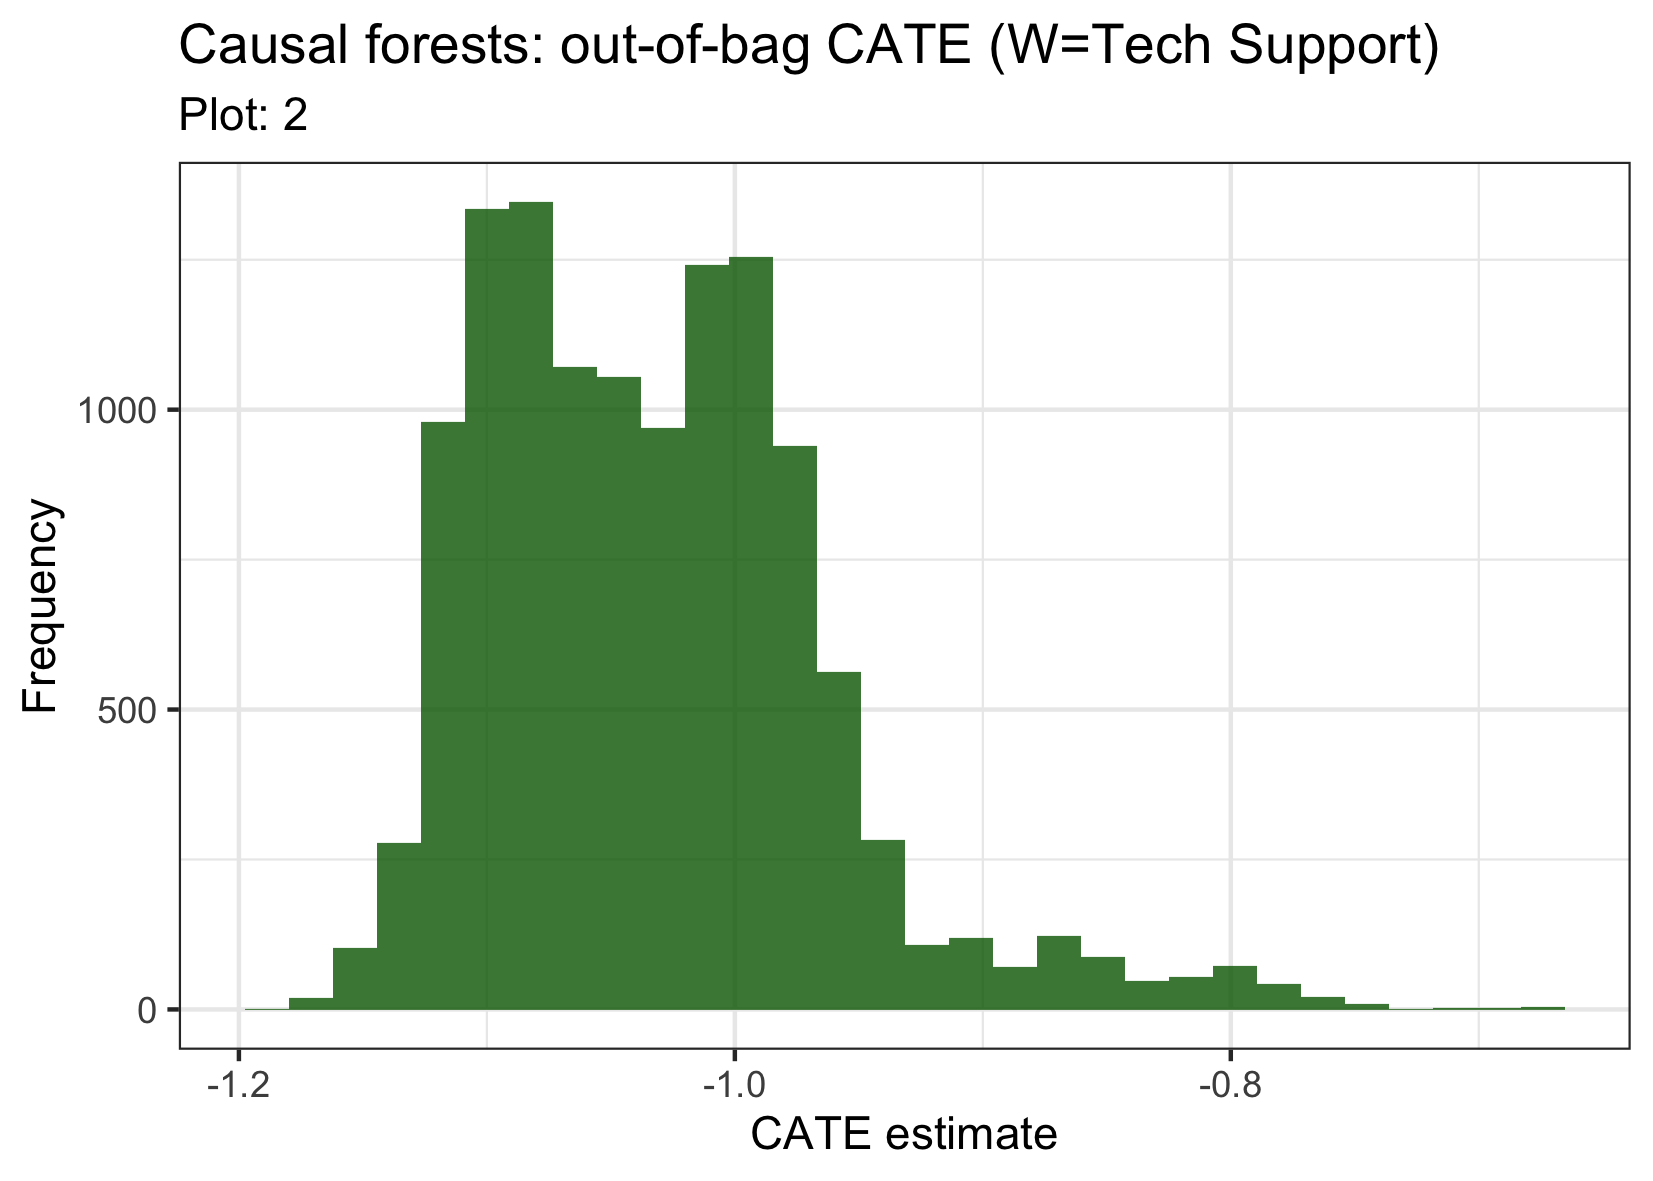
\includegraphics[scale=0.15]{chinchilab-template/chapters/appendices/ANALYSIS/CATE_2.png}
    \caption{Distribution of CATE (Model 2)}
    \label{fig:my_label}
\end{figure}


%%%%%%%%%%%%%%%%%%%%%%%%%%%%%%%%%%%%%%%%%%%%%%%%%%%%%%%%%%%%
\subsubsection{A.2.2.1 Nuisance Parameter Check}
%%%%%%%%%%%%%%%%%%%%%%%%%%%%%%%%%%%%%%%%%%%%%%%%%%%%%%%%%%%%

\begin{table}[H]{
    \begin{subtable}{.5\textwidth}
    \centering
    \scriptsize
        {\begin{tabular}{@{\extracolsep{5pt}}lc} 
        \\[-1.8ex]\hline 
        \hline \\[-1.8ex] 
         & \multicolumn{1}{c}{\textit{Dependent variable: Green Flag}} \\ 
        \cline{2-2} 
        \\[-1.8ex] &   \\ 
        \hline \\[-1.8ex] 
         e.bar & 1.000$^{***}$ \\ 
          & (0.027) \\ 
          & \\ 
         e.residual & 17.468$^{***}$ \\ 
          & (0.525) \\ 
          & \\ 
        \hline \\[-1.8ex] 
        \hline 
        \hline \\[-1.8ex] 
        \textit{Note:}  & \multicolumn{1}{r}{$^{*}$p$<$0.1; $^{**}$p$<$0.05; $^{***}$p$<$0.01} \\ 
        \end{tabular} }
    \subcaption{Outcome Model}
    \end{subtable}
    \begin{subtable}{0.3\linewidth}
    \centering
    \scriptsize
        {\begin{tabular}{@{\extracolsep{5pt}}lc} 
        \\[-1.8ex]\hline 
        \hline \\[-1.8ex] 
         & \multicolumn{1}{c}{\textit{Dependent variable: Green Flag}} \\ 
        \cline{2-2} 
        \\[-1.8ex] &   \\ 
        \hline \\[-1.8ex] 
         m.bar & 1.000$^{***}$ \\ 
          & (0.006) \\ 
          & \\ 
         m.residual & 12.864$^{***}$ \\ 
          & (0.161) \\ 
          & \\ 
        \hline \\[-1.8ex] 
        \hline 
        \hline \\[-1.8ex] 
        \textit{Note:}  & \multicolumn{1}{r}{$^{*}$p$<$0.1; $^{**}$p$<$0.05; $^{***}$p$<$0.01} \\ 
        \end{tabular}}
    \subcaption{Propensity Model}
    \end{subtable}
\caption{Calibration Regressions (Model 2)}
\label{x}}
\end{table}

\begin{figure}[H]
    \centering
    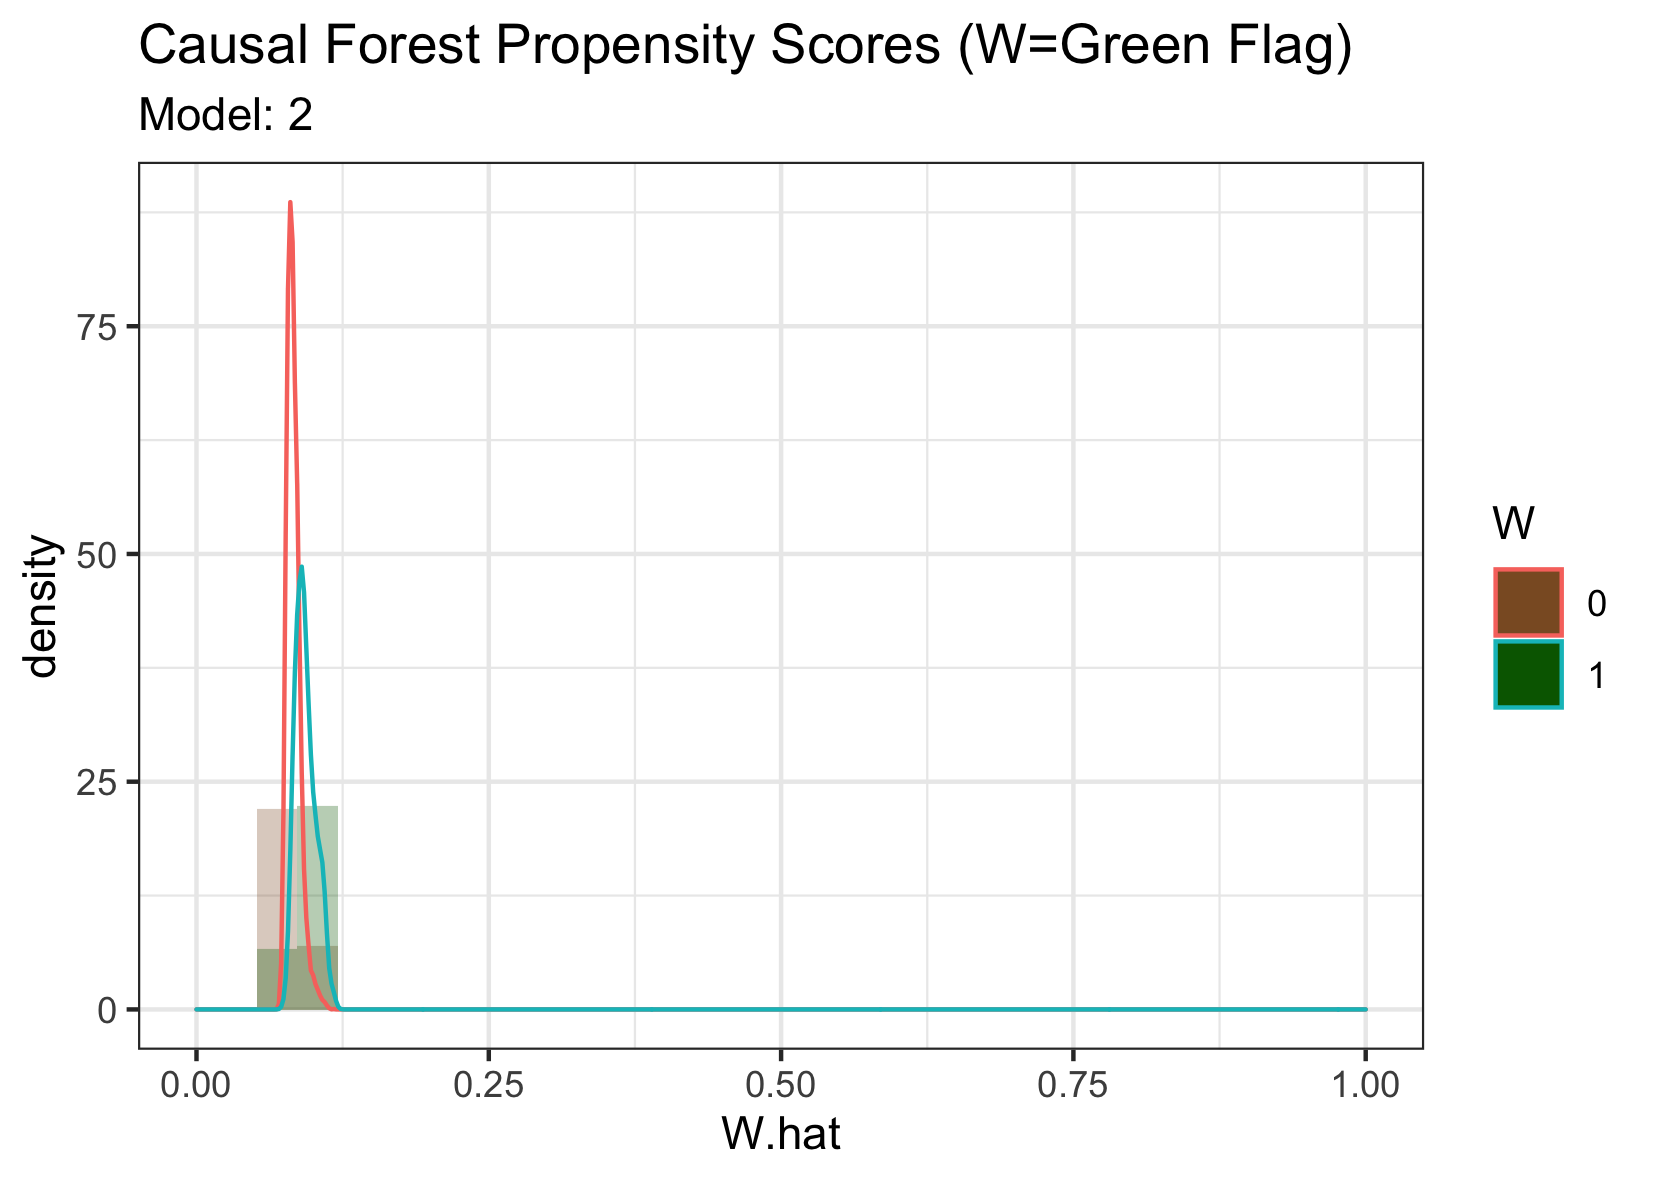
\includegraphics[scale=0.15]{chinchilab-template/chapters/appendices/ANALYSIS/prop_2.png}
    \caption{Propensity Score Distribution (Model 2)}
    \label{fig:my_label}
\end{figure}

\newpage

%%%%%%%%%%%%%%%%%%%%%%%%%%%%%%%%%%%%%%%%%%%%%%%%%%%%%%%%%%%%
\subsubsection{A.2.2.2 Heterogeneity Assessment}
%%%%%%%%%%%%%%%%%%%%%%%%%%%%%%%%%%%%%%%%%%%%%%%%%%%%%%%%%%%%
\begin{table}[h!]
\centering
\caption{Variable Importance (Model 2)}
\begin{tabular}{lr}
\\[-1.8ex]\hline 
\hline \\[-1.8ex] 
\rowcolor[HTML]{FFFFFF} 
{\color[HTML]{333333} \textbf{Covariate}} & {\color[HTML]{333333} \textbf{Value}} \\ \hline
\rowcolor[HTML]{FFFFFF} 
{\color[HTML]{333333} 2022} & \cellcolor[HTML]{00441B}{\color[HTML]{FFFFFF} 0.06224698} \\
\rowcolor[HTML]{FFFFFF} 
{\color[HTML]{333333} Issue Amount} & \cellcolor[HTML]{359E53}{\color[HTML]{FFFFFF} 0.05900688} \\
\rowcolor[HTML]{FFFFFF} 
{\color[HTML]{333333} Time to Maturity (Days)} & \cellcolor[HTML]{7FC97E}{\color[HTML]{333333} 0.05695576} \\
\rowcolor[HTML]{FFFFFF} 
{\color[HTML]{333333} Utilities} & \cellcolor[HTML]{8ACE88}{\color[HTML]{333333} 0.05664093} \\
\rowcolor[HTML]{FFFFFF} 
{\color[HTML]{333333} Annual Coupon} & \cellcolor[HTML]{CCEBC5}{\color[HTML]{333333} 0.05452951} \\
\rowcolor[HTML]{FFFFFF} 
{\color[HTML]{333333} Semi Annual Coupon} & \cellcolor[HTML]{F7FCF5}{\color[HTML]{333333} 0.05223546} \\ \hline
\end{tabular}
\end{table}

\begin{figure}[h!]
    \centering
    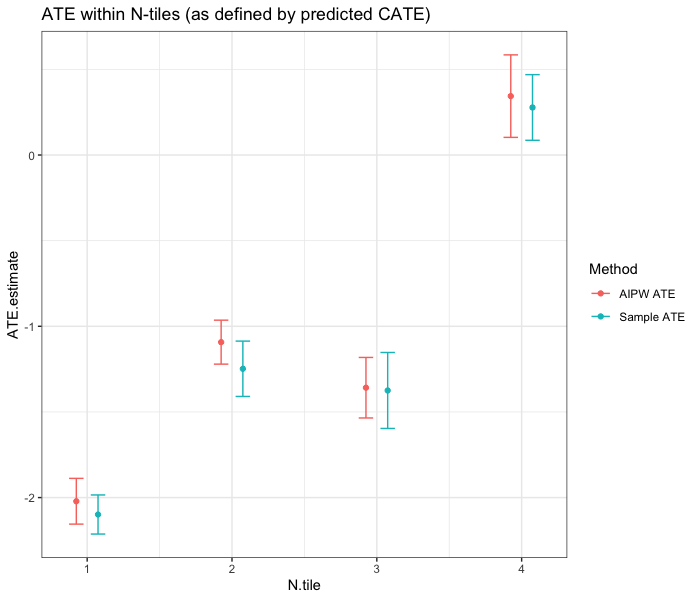
\includegraphics[scale=0.6]{chinchilab-template/chapters/appendices/ANALYSIS/ntile_cf0.1.png}
    \caption{Graph of ATE within Subgroups (Model 2)}
    \label{fig:my_label}
\end{figure}

\begin{figure}[H]
\centering
   \begin{subfigure}[b]{0.45\textwidth}
    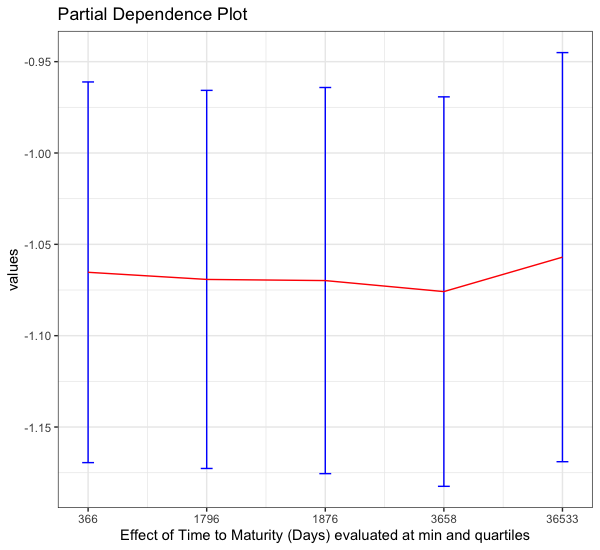
\includegraphics[width=0.9\textwidth]{chinchilab-template/chapters/appendices/ANALYSIS/PDP_cf0.1.png}
    \caption{Effect of Time to Maturity (Days)}
   \label{fig:Ng1} 
\end{subfigure}
\begin{subfigure}[b]{0.45\textwidth}
    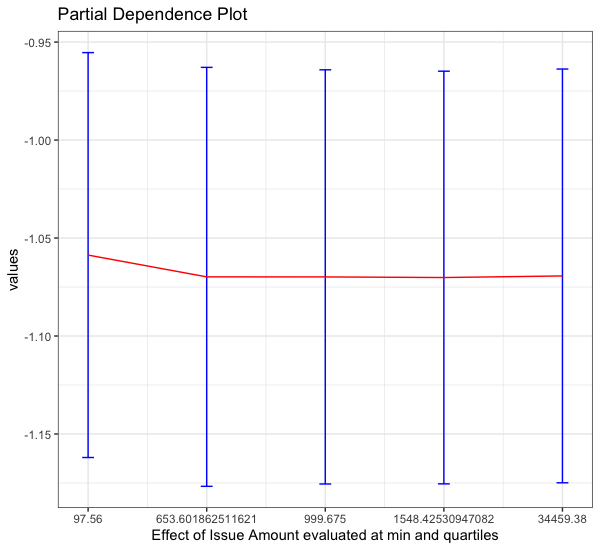
\includegraphics[width=0.9\textwidth]{chinchilab-template/chapters/appendices/ANALYSIS/PDP2_cf0.1.png}
    \caption{Effect of Issue Amount}
   \label{fig:Ng2}
\end{subfigure}
\\
\begin{subfigure}[b]{0.45\textwidth}
    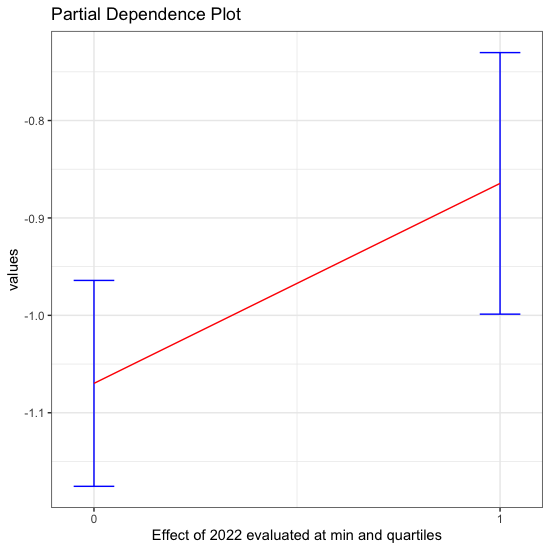
\includegraphics[width=0.9\textwidth]{chinchilab-template/chapters/appendices/ANALYSIS/PDP3_cf0.1.png}
    \caption{Effect of 2022}
   \label{fig:Ng2}
\end{subfigure}
\caption{Partial Dependency Plots (Model 2)}
\end{figure}

\begin{table}[]
\caption{Heterogeneity across Covariates (Model 2)}
\label{Het1}
\footnotesize
\begin{tabular}{lllll}
\\[-1.8ex]\hline 
\hline \\[-1.8ex] 
{\color[HTML]{333333} \textbf{Variable}} & {\color[HTML]{333333} \textbf{Mean ntile1}} & {\color[HTML]{333333} \textbf{Mean ntile2}} & {\color[HTML]{333333} \textbf{Mean ntile3}} & {\color[HTML]{333333} \textbf{Mean ntile4}} \\
\hline \\[-1.8ex] 
Time to   Maturity (Days) & \cellcolor[HTML]{63BE7B}3054.57 & \cellcolor[HTML]{C1E4CC}2681.13 & \cellcolor[HTML]{B6E0C3}2724.35 & \cellcolor[HTML]{FCFCFF}2441.21 \\
Issue Amount & \cellcolor[HTML]{63BE7B}1554.38 & \cellcolor[HTML]{B3DFC0}1410.58 & \cellcolor[HTML]{FCFCFF}1278.26 & \cellcolor[HTML]{6BC182}1541.41 \\
Guarantor & \cellcolor[HTML]{DBEFE2}0.22 & \cellcolor[HTML]{D5ECDD}0.26 & \cellcolor[HTML]{DEF0E5}0.2 & \cellcolor[HTML]{D6EDDE}0.25 \\
2013 & \cellcolor[HTML]{EDF6F2}0.1 & \cellcolor[HTML]{F5F9F9}0.05 & \cellcolor[HTML]{F0F8F5}0.08 & \cellcolor[HTML]{F5F9F9}0.05 \\
2014 & \cellcolor[HTML]{EFF7F4}0.09 & \cellcolor[HTML]{F3F9F8}0.06 & \cellcolor[HTML]{F2F8F6}0.07 & \cellcolor[HTML]{F5F9F9}0.05 \\
2015 & \cellcolor[HTML]{F3F9F8}0.06 & \cellcolor[HTML]{EFF7F4}0.09 & \cellcolor[HTML]{F2F8F6}0.07 & \cellcolor[HTML]{F3F9F8}0.06 \\
2016 & \cellcolor[HTML]{F5F9F9}0.05 & \cellcolor[HTML]{F2F8F6}0.07 & \cellcolor[HTML]{F2F8F6}0.07 & \cellcolor[HTML]{F0F8F5}0.08 \\
2017 & \cellcolor[HTML]{F6FAFA}0.04 & \cellcolor[HTML]{F2F8F6}0.07 & \cellcolor[HTML]{F2F8F6}0.07 & \cellcolor[HTML]{F3F9F8}0.06 \\
2018 & \cellcolor[HTML]{FBFCFE}0.01 & \cellcolor[HTML]{F0F8F5}0.08 & \cellcolor[HTML]{F3F9F8}0.06 & \cellcolor[HTML]{F0F8F5}0.08 \\
2019 & \cellcolor[HTML]{F5F9F9}0.05 & \cellcolor[HTML]{F0F8F5}0.08 & \cellcolor[HTML]{F2F8F6}0.07 & \cellcolor[HTML]{F3F9F8}0.06 \\
2020 & \cellcolor[HTML]{F2F8F6}0.07 & \cellcolor[HTML]{F6FAFA}0.04 & \cellcolor[HTML]{F0F8F5}0.08 & \cellcolor[HTML]{F8FBFC}0.03 \\
2021 & \cellcolor[HTML]{EDF6F2}0.1 & \cellcolor[HTML]{F6FAFA}0.04 & \cellcolor[HTML]{F2F8F6}0.07 & \cellcolor[HTML]{F8FBFC}0.03 \\
2022 & \cellcolor[HTML]{FCFCFF}0 & \cellcolor[HTML]{FCFCFF}0 & \cellcolor[HTML]{FCFCFF}0 & \cellcolor[HTML]{DFF1E6}0.19 \\
Annual Coupon & \cellcolor[HTML]{63BE7B}1 & \cellcolor[HTML]{68C07F}0.97 & \cellcolor[HTML]{D9EEE1}0.23 & \cellcolor[HTML]{E7F4ED}0.14 \\
Semi Annual   Coupon & \cellcolor[HTML]{FCFCFF}0 & \cellcolor[HTML]{F9FBFD}0.02 & \cellcolor[HTML]{88CD9B}0.76 & \cellcolor[HTML]{7AC88F}0.85 \\
Quarterly & \cellcolor[HTML]{FCFCFF}0 & \cellcolor[HTML]{FCFCFF}0 & \cellcolor[HTML]{FCFCFF}0 & \cellcolor[HTML]{FCFCFF}0 \\
Monthly & \cellcolor[HTML]{FCFCFF}0 & \cellcolor[HTML]{FCFCFF}0 & \cellcolor[HTML]{FCFCFF}0 & \cellcolor[HTML]{FCFCFF}0 \\
Variable & \cellcolor[HTML]{FCFCFF}0 & \cellcolor[HTML]{FCFCFF}0 & \cellcolor[HTML]{FCFCFF}0 & \cellcolor[HTML]{FCFCFF}0 \\
First Lien Loan & \cellcolor[HTML]{FCFCFF}0 & \cellcolor[HTML]{FCFCFF}0 & \cellcolor[HTML]{FCFCFF}0 & \cellcolor[HTML]{FCFCFF}0 \\
First Mortgage & \cellcolor[HTML]{FCFCFF}0 & \cellcolor[HTML]{FCFCFF}0 & \cellcolor[HTML]{FCFCFF}0 & \cellcolor[HTML]{FCFCFF}0 \\
First   Refunding Mortgage & \cellcolor[HTML]{FCFCFF}0 & \cellcolor[HTML]{FCFCFF}0 & \cellcolor[HTML]{FCFCFF}0 & \cellcolor[HTML]{FCFCFF}0 \\
Second Lien Loan & \cellcolor[HTML]{FCFCFF}0 & \cellcolor[HTML]{FCFCFF}0 & \cellcolor[HTML]{FCFCFF}0 & \cellcolor[HTML]{FCFCFF}0 \\
Junior   Subordinated & \cellcolor[HTML]{FCFCFF}0 & \cellcolor[HTML]{FCFCFF}0 & \cellcolor[HTML]{FCFCFF}0 & \cellcolor[HTML]{FCFCFF}0 \\
Senior   Secured Mortgage & \cellcolor[HTML]{FBFCFE}0.01 & \cellcolor[HTML]{DFF1E6}0.19 & \cellcolor[HTML]{F0F8F5}0.08 & \cellcolor[HTML]{F5F9F9}0.05 \\
Refunding   Mortgage & \cellcolor[HTML]{FCFCFF}0 & \cellcolor[HTML]{FCFCFF}0 & \cellcolor[HTML]{FCFCFF}0 & \cellcolor[HTML]{FBFCFE}0.01 \\
Senior Secured & \cellcolor[HTML]{FBFCFE}0.01 & \cellcolor[HTML]{EAF5F0}0.12 & \cellcolor[HTML]{F3F9F8}0.06 & \cellcolor[HTML]{ECF6F1}0.11 \\
Senior Unsecured & \cellcolor[HTML]{77C78D}0.87 & \cellcolor[HTML]{B8E1C4}0.45 & \cellcolor[HTML]{8ACE9C}0.75 & \cellcolor[HTML]{AEDDBC}0.51 \\
Senior Non   Preferred & \cellcolor[HTML]{F8FBFC}0.03 & \cellcolor[HTML]{F8FBFC}0.03 & \cellcolor[HTML]{FCFCFF}0 & \cellcolor[HTML]{FBFCFE}0.01 \\
Senior Preferred & \cellcolor[HTML]{F8FBFC}0.03 & \cellcolor[HTML]{F3F9F8}0.06 & \cellcolor[HTML]{FBFCFE}0.01 & \cellcolor[HTML]{F8FBFC}0.03 \\
Senior   Subordinated Unsecured & \cellcolor[HTML]{FBFCFE}0.01 & \cellcolor[HTML]{FCFCFF}0 & \cellcolor[HTML]{FBFCFE}0.01 & \cellcolor[HTML]{FCFCFF}0 \\
Senior   Subordinated Secured & \cellcolor[HTML]{FCFCFF}0 & \cellcolor[HTML]{FCFCFF}0 & \cellcolor[HTML]{FCFCFF}0 & \cellcolor[HTML]{FCFCFF}0 \\
Subordinated   Unsecured & \cellcolor[HTML]{F9FBFD}0.02 & \cellcolor[HTML]{FBFCFE}0.01 & \cellcolor[HTML]{F8FBFC}0.03 & \cellcolor[HTML]{F9FBFD}0.02 \\
Subordinated   Secured & \cellcolor[HTML]{FCFCFF}0 & \cellcolor[HTML]{FCFCFF}0 & \cellcolor[HTML]{FCFCFF}0 & \cellcolor[HTML]{FCFCFF}0 \\
Academic   \& Educational Services & \cellcolor[HTML]{FCFCFF}0 & \cellcolor[HTML]{FCFCFF}0 & \cellcolor[HTML]{FCFCFF}0 & \cellcolor[HTML]{FCFCFF}0 \\
Basic Materials & \cellcolor[HTML]{F9FBFD}0.02 & \cellcolor[HTML]{FCFCFF}0 & \cellcolor[HTML]{FBFCFE}0.01 & \cellcolor[HTML]{FBFCFE}0.01 \\
Consumer   Cyclicals & \cellcolor[HTML]{F8FBFC}0.03 & \cellcolor[HTML]{F9FBFD}0.02 & \cellcolor[HTML]{F9FBFD}0.02 & \cellcolor[HTML]{FBFCFE}0.01 \\
Consumer   Non Cyclicals & \cellcolor[HTML]{F9FBFD}0.02 & \cellcolor[HTML]{FBFCFE}0.01 & \cellcolor[HTML]{F9FBFD}0.02 & \cellcolor[HTML]{FBFCFE}0.01 \\
Energy & \cellcolor[HTML]{F9FBFD}0.02 & \cellcolor[HTML]{FCFCFF}0 & \cellcolor[HTML]{F9FBFD}0.02 & \cellcolor[HTML]{FBFCFE}0.01 \\
Financials & \cellcolor[HTML]{A5D9B4}0.57 & \cellcolor[HTML]{87CD9A}0.77 & \cellcolor[HTML]{96D3A7}0.67 & \cellcolor[HTML]{94D2A6}0.68 \\
Healthcare & \cellcolor[HTML]{FCFCFF}0 & \cellcolor[HTML]{FCFCFF}0 & \cellcolor[HTML]{FCFCFF}0 & \cellcolor[HTML]{FCFCFF}0 \\
Industrials & \cellcolor[HTML]{F3F9F8}0.06 & \cellcolor[HTML]{FBFCFE}0.01 & \cellcolor[HTML]{F9FBFD}0.02 & \cellcolor[HTML]{F9FBFD}0.02 \\
Institutions,   Associations \& Organizations & \cellcolor[HTML]{F8FBFC}0.03 & \cellcolor[HTML]{FBFCFE}0.01 & \cellcolor[HTML]{F6FAFA}0.04 & \cellcolor[HTML]{FBFCFE}0.01 \\
Real Estate & \cellcolor[HTML]{FBFCFE}0.01 & \cellcolor[HTML]{FCFCFF}0 & \cellcolor[HTML]{FBFCFE}0.01 & \cellcolor[HTML]{FCFCFF}0 \\
Technology & \cellcolor[HTML]{F8FBFC}0.03 & \cellcolor[HTML]{FCFCFF}0 & \cellcolor[HTML]{FBFCFE}0.01 & \cellcolor[HTML]{FBFCFE}0.01 \\
Utilities & \cellcolor[HTML]{FCFCFF}0 & \cellcolor[HTML]{FCFCFF}0 & \cellcolor[HTML]{F6FAFA}0.04 & \cellcolor[HTML]{F2F8F6}0.07 \\
AAA & \cellcolor[HTML]{EDF6F2}0.1 & \cellcolor[HTML]{A7DAB6}0.56 & \cellcolor[HTML]{D5ECDD}0.26 & \cellcolor[HTML]{B0DDBD}0.5 \\
AA & \cellcolor[HTML]{D5ECDD}0.26 & \cellcolor[HTML]{D9EEE1}0.23 & \cellcolor[HTML]{E6F3EC}0.15 & \cellcolor[HTML]{D6EDDE}0.25 \\
A & \cellcolor[HTML]{CDE9D7}0.31 & \cellcolor[HTML]{EFF7F4}0.09 & \cellcolor[HTML]{D5ECDD}0.26 & \cellcolor[HTML]{ECF6F1}0.11 \\
BBB & \cellcolor[HTML]{D2EBDB}0.28 & \cellcolor[HTML]{EFF7F4}0.09 & \cellcolor[HTML]{D8EEE0}0.24 & \cellcolor[HTML]{F0F8F5}0.08 \\
BB & \cellcolor[HTML]{F8FBFC}0.03 & \cellcolor[HTML]{F9FBFD}0.02 & \cellcolor[HTML]{F5F9F9}0.05 & \cellcolor[HTML]{F5F9F9}0.05 \\
B & \cellcolor[HTML]{FBFCFE}0.01 & \cellcolor[HTML]{FBFCFE}0.01 & \cellcolor[HTML]{F6FAFA}0.04 & \cellcolor[HTML]{F9FBFD}0.02 \\
\hline \\[-1.8ex] 
\end{tabular}
\end{table}

\begin{table}[H]
\centering
\caption{Heterogeneity across Covariates cont. (Model 2)}
\label{Het1}
\footnotesize
\begin{tabular}{lllll}
\\[-1.8ex]\hline 
\hline \\[-1.8ex] 
{\color[HTML]{333333} \textbf{Variable}} & {\color[HTML]{333333} \textbf{Mean ntile1}} & {\color[HTML]{333333} \textbf{Mean ntile2}} & {\color[HTML]{333333} \textbf{Mean ntile3}} & {\color[HTML]{333333} \textbf{Mean ntile4}} \\
\hline \\[-1.8ex] 
AUD & 0 & 0 & \cellcolor[HTML]{FBFCFE}0.01 & \cellcolor[HTML]{F9FBFD}0.02 \\
BRL & 0 & 0 & 0 & 0 \\
CAD & 0 & 0 & \cellcolor[HTML]{FBFCFE}0.01 & \cellcolor[HTML]{F8FBFC}0.03 \\
CLP & 0 & 0 & 0 & 0 \\
CNY & 0 & 0 & 0 & 0 \\
COP & 0 & 0 & 0 & 0 \\
HRK & 0 & 0 & 0 & 0 \\
EUR & \cellcolor[HTML]{6DC283}0.94 & \cellcolor[HTML]{8BCF9E}0.74 & \cellcolor[HTML]{E4F3EA}0.16 & \cellcolor[HTML]{EAF5F0}0.12 \\
GBP & \cellcolor[HTML]{F8FBFC}0.03 & \cellcolor[HTML]{EDF6F2}0.1 & \cellcolor[HTML]{F6FAFA}0.04 & \cellcolor[HTML]{F6FAFA}0.04 \\
HKD & 0 & 0 & 0 & 0 \\
JPY & 0 & 0 & \cellcolor[HTML]{F9FBFD}0.02 & \cellcolor[HTML]{EFF7F4}0.09 \\
KZT & 0 & 0 & 0 & 0 \\
MXN & 0 & 0 & 0 & 0 \\
NZD & 0 & 0 & 0 & 0 \\
NOK & 0 & 0 & 0 & 0 \\
PEN & 0 & 0 & 0 & 0 \\
PHP & 0 & 0 & 0 & 0 \\
RUB & 0 & 0 & 0 & 0 \\
SGD & 0 & 0 & 0 & 0 \\
SEK & 0 & 0 & 0 & 0 \\
CHF & 0 & \cellcolor[HTML]{FBFCFE}0.01 & \cellcolor[HTML]{F9FBFD}0.02 & 0 \\
THB & 0 & 0 & 0 & 0 \\
TRY & 0 & 0 & 0 & 0 \\
UYU & 0 & 0 & 0 & 0 \\
\hline \\[-1.8ex] 
\end{tabular}
\end{table}

\newpage